\documentclass[a4paper, 11pt]{book}
\usepackage{graphicx}
\usepackage[frenchb]{babel}
\usepackage[utf8]{inputenc} % Required for inputting international characters
\usepackage[T1]{fontenc} % Output font encoding for international characters
%\usepackage[francais]{babel}
\usepackage[french]{minitoc}
\usepackage{color}
\usepackage[noend]{algpseudocode}
\usepackage{subcaption,amsbsy,booktabs,adjustbox} 
\usepackage{frame, caption}
\usepackage{amsmath}
\usepackage{eulervm}
\usepackage{mathrsfs}
\usepackage{multirow, enumitem, longtable, rotating,lipsum, scrextend}
\usepackage{array}
\usepackage{floatflt}
\usepackage{makecell}
\usepackage{xcolor, soul}
\sethlcolor{yellow}	
\usepackage{floatrow}
\usepackage{setspace}
\usepackage{fontenc}
\usepackage{xcolor, soul}
\sethlcolor{yellow}	
\usepackage{floatrow}
\usepackage{setspace}
\newcommand{\argmax}{\operatornamewithlimits{arg\,max}}







\begin{document}
	
%	\tableofcontents
	\chapter{État de l'art }
	%What is dominance in social psychology
%Nonverbal Behavior and the Vertical Dimension of Social Relations: A Meta-Analysis
%
%\textbf{several representation of dominance :} 
%For example, dominance can be defined as a personality trait involving the motive to control others, the self-
%perception of oneself as controlling others, and/or as a behavioral
%outcome (success in controlling others or their resources). Status,
%involving an ascribed or achieved quality implying respect and
%privilege, does not necessarily include the ability to control others
%or their resources.
%
% Similarly, power defined as the capacity or
%structurally sanctioned right to control others or their resources
%does not necessarily imply prestige or respect. Other distinctions
%have also been drawn, including different functional bases of
%power, such as reward power, expert power, referent power, or
%coercive power (French and Raven, 1959), and outcome dependency
%(Stevens  Fiske, 2000). Some writers conceptualize dominance
%in terms of social skill (e.g., Burgoon  Dunbar, 2000; Byrne,
%2001). Some writers define dominance as the enactment of certain
%nonverbal or verbal behaviors (Rosa  Mazur, 1979). Authors do
%not use the various verticality terms such as power, dominance,
%and status in consistent ways, and often the terms are used without
%a clear definition.
%
%\textbf{Burgoon and dunber 2010}
%

%
%
%La dominance, d'un autre côté, se réfère à des comportements interactionnels dépendant du contexte et de la relation, dans lesquels le pouvoir est rendu saillant et l'influence est atteinte %(Burgoon et al., 1998; Mack, 1974; Rogers-Millar & Millar, 1979)
%dans le contexte de l'échange interpersonnel, la dominance est basée sur une combinaison de tempérament individuel et de caractéristiques situationnelles qui encouragent un comportement dominant. 
%Le dominance interpersonnelle est un comportement de communication basé sur la relation qui dépend du contexte et des motivations des individus impliqués
%
 
%Comme l'ont noté Emerson (1962) et d'autres théoriciens, le pouvoir équivaut à dépendre des autres et suppose donc une relation sociale.
%
%\textbf{Dyadic power theory:}
%
%
%Elle se base sur les échanges sociaux de pouvoir sur 4 éléments
%
%\begin{enumerate}
%	\item cette définition s'étend pour prendre en compte les échanges sociaux qui inclut les stratégies de communications qui deviennent manifestes durant l'interaction
%	\item Contrôle relationnel : elle reconnaît que l'autorité d'utiliser ou d'échanger des ressources dans les interactions est souvent accordée aux individus par les normes sociétales ainsi que par l'histoire relationnelle propre aux individus impliqués dans l'interaction.
%	
%	\item Cette représentation insiste sur l'idée que le pouvoir doit être vu relativement, ou par rapport aux autres. Ainsi, il reconnaît que le pouvoir est une construction dynamique et multidimensionnelle qui incorpore les perspectives des deux individus dans l'interaction.
%	\item En cohérence avec une perspective de communication, il place l'interaction elle-même au centre des préoccupations. Les tentatives de prendre le contrôle de toute interaction donnée par la dominance, bien que déterminées par le pouvoir, sont au centre de la théorie car elles déterminent le résultat du processus  (la décision finale qui a des ramifications pour l'avenir de la relation).
%%\end{enumerate}
%
%
%
%
%\textbf{Interpersonal dominance paper}
%En préface, notre intention n'est pas de représenter les trois comme des perspectives exhaustives ou mutuellement exclusives sur la construction de la domination-soumission, mais plutôt de mettre en lumière les nombreuses facettes de cette dimension fondamentale des relations humaines.


\subsection{Trait de personnalité}
%Les chercheurs qui se sont intéressés à l'étude de la personnalité tendent à voir la personnalité comme stable \cite{burgoon2006nonverbal} et par conséquent, cherchent a définir des indicateurs de dominance stable permettant de de former  des profils comportementaux stables. 

La dominance comme trait de personnalité a connu une évolution où la littérature en psychologie a élargit le concept de la dominance au-delà des comportements d'agressivité.
En effet, les travaux en Éthologie et psychologie évolutive ont d'abord étudié la dominance comme un trait de personnalité innée qui confère à la personne la capacité d'exercer son pouvoir et sa domination, susciter la déférence et l'acquiescement, ou apaiser et se soumettre à un comportement conspécifique plus fort \cite{keltner1995signs,burgoon2006nonverbal}. Cependant, les travaux en Éthologie contemporaine s'éloignent de cette définition en faveur d'études pour la compréhension de l'interaction entre les organismes et leur environnement social \cite{burgoon2006nonverbal}.

Pour les psychologues de la personnalité, la dominance est considérée comme un trait individuel durable qui désigne le tempérament de la personne et les prédispositions comportementales de chacun \cite{cattell1970handbook,ridgeway1987nonverbal} tels que l'agression, l'ambition, l'argumentation,
assertivité, vantardise, confiance et détermination.
Les adjectifs communs utilisés pour décrire la personne dominante sont affirmés, agressifs, compétitifs, exigeant, égoïste et têtu. Plus précisément, la dominance en tant que variable de personnalité «montre un ajustement réaliste constant au succès et à l'échec de l'individu, à la santé ou à la maladie, aux capacités ou handicaps et aux forces extérieures relatives» \cite{cattell1970handbook,burgoon1998nature}.
En effet, selon  Emmons et McAdams \cite{emmons1991personal}, les individus avec un motif de haut pouvoir sont décrits comme voulant contrôler et influencer les autres, désirant la célébrité ou l'attention du public, et ayant la capacité de susciter l'émotion chez les autres. Dans la même veine, \cite{jackson1974personality} décrivent une personne dominante comme une personne qui cherche et maintient un rôle de leader dans un groupe. Ces personnes prennent en charge et guident les membres du groupe vers la réalisation d'objectifs louables à travers des tactiques d'influence, des manœuvres de contrôle de l'environnement et l'expression énergique de l'opinion \cite{burgoon1998nature}. 
A l'opposé, les individus non dominants ou soumis sont présentés comme coopératifs, modestes et obéissants, mais aussi obséquieux, doux, faibles, peu sûrs et évitant les situations qui nécessitent une affirmation de soi \cite{burgoon1998nature}. 

%Les habiletés sociales font partie de cette équation, car la capacité d'être énergique, de prendre des initiatives et d'être expressif mais détendu et équilibré \cite{burgoon2006nonverbal}. 
Par ailleurs, la dominance et soumission sont généralement révélés à travers le style de communication \cite{burgoon1998nature}. Une personne dominante va avoir plus d'assurance dans sa manière de communiquer, à être plus confiante, enthousiaste, énergique, active, compétitive, sûre d'elle, vaniteuse et direct. Ceci transparaît dans les comportements verbaux et non verbaux utilisés. Une personne dominante va  utiliser plus d'espace, avec un temps de conversation plus long et être capable d'avoir plus d'interruption réussies \cite{burgoon1998nature}. 

En revanche, une personne soumise va utiliser un mouvement contraint, une utilisation limitée de l'espace, de grandes quantités de regard tout en écoutant  \cite{burgoon1998nature}. Ces comportements sont présentés plus en détails dans la section ... 


\subsection{Statut social}

	Le statut et le pouvoir sont étroitement liés et parfois confondus \cite{burgoon1998nature}. Pour les sociologues, le statut désigne la position d'une personne dans une hiérarchie sociale \cite{ellyson1985power}, ce qui est répandu dans tous les types de sociétés \cite{lips1991women}.
	Ceci est confirmé  dans la littérature éthologique qui fait l'hypothèse unificatrice que la dominance représente une caractéristique universelle de l'organisation sociale reflétée dans le rang ou la position dans une hiérarchie sociale \cite{burgoon1998nature} et l'accès préférentiel aux ressources \cite{liska1990dominance}.
	
	Ces comportements ont d'abord été observé chez les primates. En effet, lorsque la concurrence pour l'accès prioritaire à la ressource s'installe entre des individus ou des groupes qui ne se connaissent pas, le classement de dominance des individus doit être établi et signalé \cite{burgoon1998nature}. Les membres des groupes primates savent tous où ils se situent et qui a le statut le plus élevé ou le plus de dominance \cite{smither1993authoritarianism}.
	L'universalité de ces signaux  dans les hiérarchies de dominance sociale communes dans les groupes de primates sont également communes dans les groupes humains \cite{burgoon1998nature}.
	
	Deux formes alternatives de dominance ont été identifiées dans la littérature.
	La première forme est la dominance acquise \cite{liska1990dominance}. Elle est associée à des facteurs tels que l'héritabilité, l'âge et l'ordre de naissance qui confèrent un plus grand contrôle ou un meilleur accès à des ressources privilégiées \cite{cattell1970handbook}.
	Par ailleurs, chez les humains, la dominance acquise est souvent assimilée à des rôles sociaux qui peut se manifester par des caractéristiques immuables \textit{(signaux statiques)} ou des indicateurs qui changent lentement \textit{(signaux lents)} de facteurs tels que la position dans une hiérarchie de statut, l'âge, la maturité, la parenté, l'ordre de naissance, et rôles institutionnalisés \cite{burgoonnonverbal}. 
	
	La seconde forme est la dominance sociale \cite{liska1990dominance}, qui est acquise à travers des capacités, des stratégies ou des possibilités d'affiliation démontrées \cite{burgoon1998nature}. Contrairement au caractère immuable des manifestations de domination acquise, la dominance sociale peut se manifester par des indicateurs dynamiques tels que la proximité, la posture, le regard, l'expression faciale, la vocalisation, la durée de la conversation ou l'usage de la langue \cite{keating1985human}. Elle se révèle être particulièrement pertinente pour ceux qui s'intéressent à la communication interpersonnelle, de tels affichages peuvent être liés par les relations, les contextes et le temps\cite{burgoon1998nature}.
		
	Un statut élevé accorde un certain degrés de pouvoir et peut faciliter la dominance parce qu'on est doté d'une autorité légitime, et l'autorité légitime confère à l'individu le potentiel d'une plus grande influence \cite{burgoon2006nonverbal}. 
	
	Cependant, un statut élevé ne garantit pas l'exercice du pouvoir ou l'affichage d'un comportement dominant, et les manifestations de dominance en l'absence de pouvoir légitime peuvent ne pas réussir à exercer une influence \cite{ridgeway1995legitimacy}.
	Par ailleurs, les individus de haut rang ne sont pas forcément puissants ou dominants et les démonstrations de dominance ne placent inévitablement pas haut dans une hiérarchie de statut\cite{burgoonnonverbal}.
	
	\subsection{Relation interpersonnelle}
		Burgoon \emph{et al} \cite{burgoon1998nature} défendent le concept de la dominance et la soumission comme propriétés d'une relation interpersonnelle plutôt que individuelle, et mettent l'accent sur les habiletés sociales et les pratiques de communication qui contribuent à la dominance plutôt que sur les comportements hérités, biologiquement déterminés, contrôlés par la personnalité.
		
		Cependant, la relation interpersonnelle de dominance est souvent confondue avec le pouvoir. Étant fortement corrélés \cite{dunbar2005perceptions}, ils sont souvent regroupés sous une même rubrique \cite{ellyson1985power} et souvent utilisés comme synonymes.
		
		Plusieurs recherches en psychologie sociale \cite{burgoon1998nature,dunbar2005perceptions} se sont intéressés à définir clairement la relation interpersonnelle de dominance, le pouvoir et la relation entre ces deux concepts. 
		
		
		La définition du pouvoir est  restée longtemps conflictuelles dans les différents domaines d'applications. Cependant, la littérature en psychologie sociale et en communication interpersonnelle, converge à définir le pouvoir comme la capacité à produire les effets voulus et, en particulier, la capacité d'influencer le comportement d'une autre personne même face à la résistance  \cite{burgoon2000interactionist,burgoon2006nonverbal,huston1983power}
	
		\emph{Burgoon et Dunbar} \cite{burgoon1998nature,dunbar2005perceptions} ajoutent que comme le pouvoir est une capacité, il est latent. Par conséquent, il n'est pas toujours exercé et une personne puissante peut ne pas avoir conscience de son pouvoir. De plus, quand il est exercé, il n'est pas toujours couronné de succès et même réussi, il peut avoir une magnitude limitée en fonction de l'environnement \cite{huston1983power}.
		
		
		Les spécialistes de la communication et de la psychologie sociale considèrent en grande partie la dominance comme une variable sociale plutôt qu'organismique, mais qui est définie au niveau interpersonnel. Par ailleurs, la dominance et la soumission sont placés dans le contexte des partis multiples, c'est à dire que la dominance est une variable dyadique plutôt que monadique et est définit en fonction des résultats auxquels elle se rapporte  \cite{burgoon1998nature,burgoon2006nonverbal}.
	
		Comme l'écrivent \emph{Mitchell et Maple} \cite{smither1993authoritarianism}, la dominance est le résultat d'une interaction d'événements et dépend donc des individus impliqués dans l'interaction et non de l'individu seul.
		
	 	Contrairement au pouvoir qui peut être latent, la dominance est forcément manifeste et comportementale, elle consiste en des stratégies expressives, basées sur la relation. Elle s'exprimer par un ensemble de transactions complémentaires à travers des actes communicatifs par lesquels l'influence est exercée et accueillie avec acquiescement d'un autre \cite{burgoon2000interactionist,millar1987relational}. 
		
		De plus, même si la soumission-dominance est conceptualisée comme une dimension universelle sur laquelle toutes les relations sociales peuvent être réparties, l'expression de dominance peut être provoquée par une combinaison de tempéraments individuels et de caractéristiques situationnelles	qui encouragent un comportement dominant \cite{burgoon2000interactionist}. Ces derniers, sont sensibles à l'évolution des objectifs, des interlocuteurs, des situations et du temps, entre autres facteurs.
		Ainsi, au cours d'un même épisode, les individus peuvent ajuster leurs expressions de soumission de dominance à des circonstances changeantes.
		
		Comme nous l'avons expliqué plus haut, la dominance et le pouvoir sont deux concepts distincts. Cependant, cette présentation démontre aussi une forte corrélation entre eux. 
		Par exemple, \emph{Burgoon et Dillman} \cite{burgoon1995interpersonal} soutiennent que la dominance n'est qu'un moyen pour exprimer le pouvoir et d'atteindre l'influence voulue.
		Ils ajoutent que la dominance n'est donc pas la voie exclusive du pouvoir, mais plutôt l'un des moyens alternatifs par lesquels le pouvoir est opéré. D'un autre coté, le pouvoir fournit le contexte pour les comportements de dominance. %Par conséquent, elle ne doit pas être considérée comme synonyme de pouvoir %Keltner, Gruenfeld,  Anderson, 2003).
		
		Une autre distinction est que le pouvoir se réfère souvent à de simples potentialités d'influence (telles que reflétées dans des concepts comme les bases de pouvoir, les motivations de pouvoir et le locus de contrôle),
		alors que la dominance est plus souvent liée au comportements réels \cite{dunbar2005perceptions,burgoon1998nature}. 
		Ainsi, alors que le pouvoir permet l'affichage de la dominance, et que le comportement dominant peut solidifier le pouvoir, la dominance et le pouvoir, bien que corrélés, ne sont pas des concepts interchangeables \cite{burgoon1995interpersonal}.
		
		Enfin, la dominance et le pouvoir, appliqués à un contexte social, sont relatifs au partenaire social et ne sont pas absolus \cite{dunbar2005perceptions}.
		
	\subsection{Conclusion}
		Converger vers le fait que nous nous intéressons à la relation interpersonnelle dans le cadre d'une négociation collaborative avec un agent conversationnel.
	\section{Manifestations de la dominance dans les interactions}
		La relation interpersonnelle de dominance se manifeste à travers des actes communicatifs durant l'interactions. Ces actes sont produits soit à travers des comportements verbaux ou non verbaux.
		Nous présentons dans cette section, les comportements communicatifs liés à la relation de dominance. 
		\subsection{Comportements verbaux}
		
		\subsection{Comportements non-verbaux}
			Les indicateurs non verbaux de dominances sont riches et ont été longtemps étudié \cite{burgoon1995interpersonal,burgoon1998nature}. Une manière de diviser les indices non verbaux est par le code général utilisé pour les classer (tels que kinésique, vocalique, proxémique, haptique, etc.) \cite{burgoon2006nonverbal}. En effet, Dunbar et Burgoon \cite{dunbar2005perceptions} résume qu'un communicateur non verbal dominant prototypique serait plus dynamique sur le plan kinésique et vocal (en utilisant plus de gestes, plus de regard, plus d'animation vocale et plus de bavardages) tout en donnant l'impression de relaxation et de confiance .
			
			 Les indices kinésiques étant les plus riches (expression faciale, direction du regard, posture, mouvements corporels et gestes \emph{etc.}).
			Par exemple, Dunbar et Burgoon \cite{dunbar2005perceptions} ont constaté que plus une femme avait un contrôle corporel, plus elle était perçue comme dominante par les observateurs. De plus, les personnes en position de pouvoir  étaient les plus expressifs et  contrôlaient de leur corps. Dans la même veine,  Carney\emph{et al}\cite{hall2005nonverbal} ont constaté que les individus de grande puissance étaient perçus comme se penchant en avant, avaient des positions ouvertes, s'orientaient vers l'autre et avaient une posture plus érigée que ceux de moindre puissance. Par ailleurs, les gestes se rapportent aussi à la perception de dominance.  Carney\emph{et al}  \cite{hall2005nonverbal} ont constaté que les personnes de grande puissance étaient plus susceptibles d'utiliser des gestes, de déclencher plus de tremblements de la main et d'avoir une plus grande fréquence de contact invasif. Dunbar et Burgoon \cite{dunbar2005perceptions} ont constaté que les observateur considéraient les hommes avec une utilisation accrue des gestes d'illustrations comme étant plus dominants.
			
			Le regard apporte aussi un impact sur la perception de la dominance. Dunbar et Burgoon \cite{dunbar2005perceptions} ont constaté que des rapports de dominance visuelle plus élevés étaient corrélés à une dominance plus élevée perçue. En outre, Carney\emph{et al} \cite{hall2005nonverbal} ont trouvé que le regard plus mutuel, plus long, et regarder son interlocuteur en parlant seraient plus appropriés venant d'un individu avec plus de dominance.
			
			Les indicateurs de dominance vocaux incluent la fréquence et la longueur de temps de parole \cite{mast2002dominance}, le volume de la parole, le tempo de la parole, la hauteur, le contrôle vocal, et les interruptions \cite{dunbar2005perceptions}.
		
		\subsection{Conclusion}
\section{Négociation et dominance}
Negotiation has been defined as "an interpersonal
decision-making process by which two or
more people agree how to allocate scarce resources" \cite{thompson2000mind}

Intro de négociation et pouvoir %https://msbfile03.usc.edu/digitalmeasures/kimpeter/intellcont/Power%20dynamics%20in%20negotiation%20(AMR,%202005)-1.pdf



	\minitoc
%	\chapter{Modèle de négociation collaborative}
%		\minitoc
%%		
%		% !TeX spellcheck = fr_FR
	
	Comme mentionné dans l'introduction, la principale contribution de cette thèse est d'étudier l'impact de la relation de dominance sur les stratégies de négociation dans le cadre de négociation collaborative entre un agent conversationnel et un utilisateur humain. 
	Pour ce faire, nous devons construire un modèle de négociation qui permettent aux négociateurs de présenter leurs stratégies de négociation. 
	
	Dans ce chapitre, nous présentons notre modèle de négociation collaborative sur lequel sera construit notre modèle de décision basé sur la dominance. 
	
	Afin de définir un système de dialogue dans lequel la relation de dominance régit le choix du prochain énoncé, nous avons d'abord enregistré des dialogues de négociation entre deux personnes afin d'observer leurs comportements dans un cadre de dialogue social de type "négociation collaborative". Nous avons annotés et analysé les dialogues. Cette étude nous a livré un ensemble de comportements  que nous présenterons dans la première section de ce chapitre. 
	
	Les informations collectées grâce l'observation des comportements humains nous a guidés dans la conception de notre modèle de négociation.
	
	
	
	Dans la seconde section, nous présenterons le domaine de négociation utilisé. Dans le cadre de cette thèse, nous nous basons sur les modèles de négociations multi-critères largement utilisé dans la mise en œuvre de systèmes de négociations automatiques. 
	
	La troisième section présentera notre modèle de communication basé sur des actes de dialogues. En effet, nous nous sommes réapproprié les actes de dialogue de \cite{grosz1986attention} pour la négociation collaborative.
	
	
	 \section{Collecte de données}
		 Afin de définir un système de dialogue social dans lequel la relation de dominance régit le choix du prochain énoncé, nous avons d'abord effectuer une étude dans laquelle nous avons analyser les comportements de deux interlocuteurs dans un cadre de dialogue social de type "négociation collaborative". 
		Le but du dialogue est de trouver un restaurant où dîner avec son interlocuteur. De plus, les interlocuteurs n'avaient pas de connaissances prérequis sur les préférences de leur interlocuteur.
		
		Une fois le dialogue enregistré, nous les avons annoté et analyser la structure du dialogue en suivant la théorie de \emph{Grosz et Sidner} \cite{sidner1994artificial} qui stipule que la structure du dialogue est composée de trois éléments à savoir la structure linguistique, la structure intentionnelle et enfin l'état attentionnel.	
		Nous présenterons dans ce qui suit la procédure de l'analyse ainsi que les résultats obtenus. 
		
		\subsection{Analyse de la structure de dialogue}  
			La théorie présenté par \emph{Grosz et Sidner} propose que la structure d'un dialogue orienté tâche est constituée de trois éléments, chacun agissant sur un aspect du dialogue. 
			
			D'abord, \emph{la structure linguistique} a pour but de décomposer le dialogue en une séquence de segments de dialogue appelé (\textit{DS: discourse segment }) de tel sorte que chaque segment est composé d'un ensemble de sous-segments et d'une séquence d'énoncés appartenant uniquement au segment(n'appartient pas a un sous segment). De plus, les énoncés au sein d'un même segment contribuent à un même but. Cette décomposition est non strict du fait qu'il est difficile de trouver des indices de segmentation. Des exemples d'indices proposés sont l'intention communicative commune à chaque DS, des expressions  linguistiques comme l'utilisation de termes "d'abord, finalement, $\ldots$". Des indices plus subtiles tels que le changement d'intonation, le temps de pause peuvent aussi être utilisés.
			
	%	\subsection{Structure intentionnelle}
			Ensuite vient \emph{la structure intentionnelle}. En effet, un interlocuteur s'engage dans un dialogue poussé par une ou plusieurs intentions internes qu'on nomme \emph{DP: discourse purpose}. De plus, pour chaque \emph{DS}, nous pouvons isolé un but spécifique noté \emph{DSP: Discourse segment purpose}. Le but est d'analyser comment les\emph{ DSPs} participent à la satisfaction du \emph{DS} initial. En outre, cette structure comprend l'analyse des relations entre les différents \emph{DSPs}. Deux relations ont été identifiées, \emph{dominance} et \emph{satisfaction-precedence}. Si la satisfaction de l'intention d'un \emph{DSP1} participe a la satisfaction de celle d'un \emph{DSP2}, alors le \emph{DSP1} \textbf{contribue} au \emph{DSP2}. Par opposition le \emph{DSP2} \textbf{domine} le \emph{DSP1}.
	
			
			Finalement, \emph{l'état attentionnel} s'intéresse à l'abstraction de l'attention des participants au fur et à mesure que leur dialogue avance \cite{sidner1994artificial}. Il est défini avec une pile dynamique \emph{focus stack} qui enregistre les objets, propriétés et les intentions saillantes  à un moment donné dans le dialogue. Le processus de manipulation des espaces dans le dialogue sur la pile attentionnelle (\emph{focus stack}). Cette pile est aussi utilisé pour faciliter l'identification des relations entre les différents \emph{DSPs}
			
%			% Dynamic stack that records salient objects, properties and relations Focusing – process of manipulating focus spaces on attentional (focus) stack
%			 Focus space: les entités saillantes du dilaogue

		 \subsection{Exemple de l'analyse}
			 Nous présentons dans cette section un exemple de l'analyse dite en DSP que nous avons effectué sur un dialogue préalablement enregistré. Le texte a été édité afin d'améliorer son intelligibilité en supprimant les pauses et des mots tels que "hmm, oué $\ldots$".
			 
			 D'abord, nous nous sommes intéressés à la structure linguistique. En effet, nous avons extrait les actes de dialogues de chaque tour de dialogue, que nous avons ensuite regroupé en \emph{DS}. 
			 
			 La seconde étape consistait à analyser le but ou l'intention caché derrière chaque \emph{DS}. Par conséquent, nous avons formulé les \emph{DSPs} comme présenté dans l'exemple ci-dessus. L'état attentionnel nous a aidé à la construction des différents \emph{DS} et a formuler les intentions pour chaque \emph{DSP}	
			
			
			\begin{figure}
				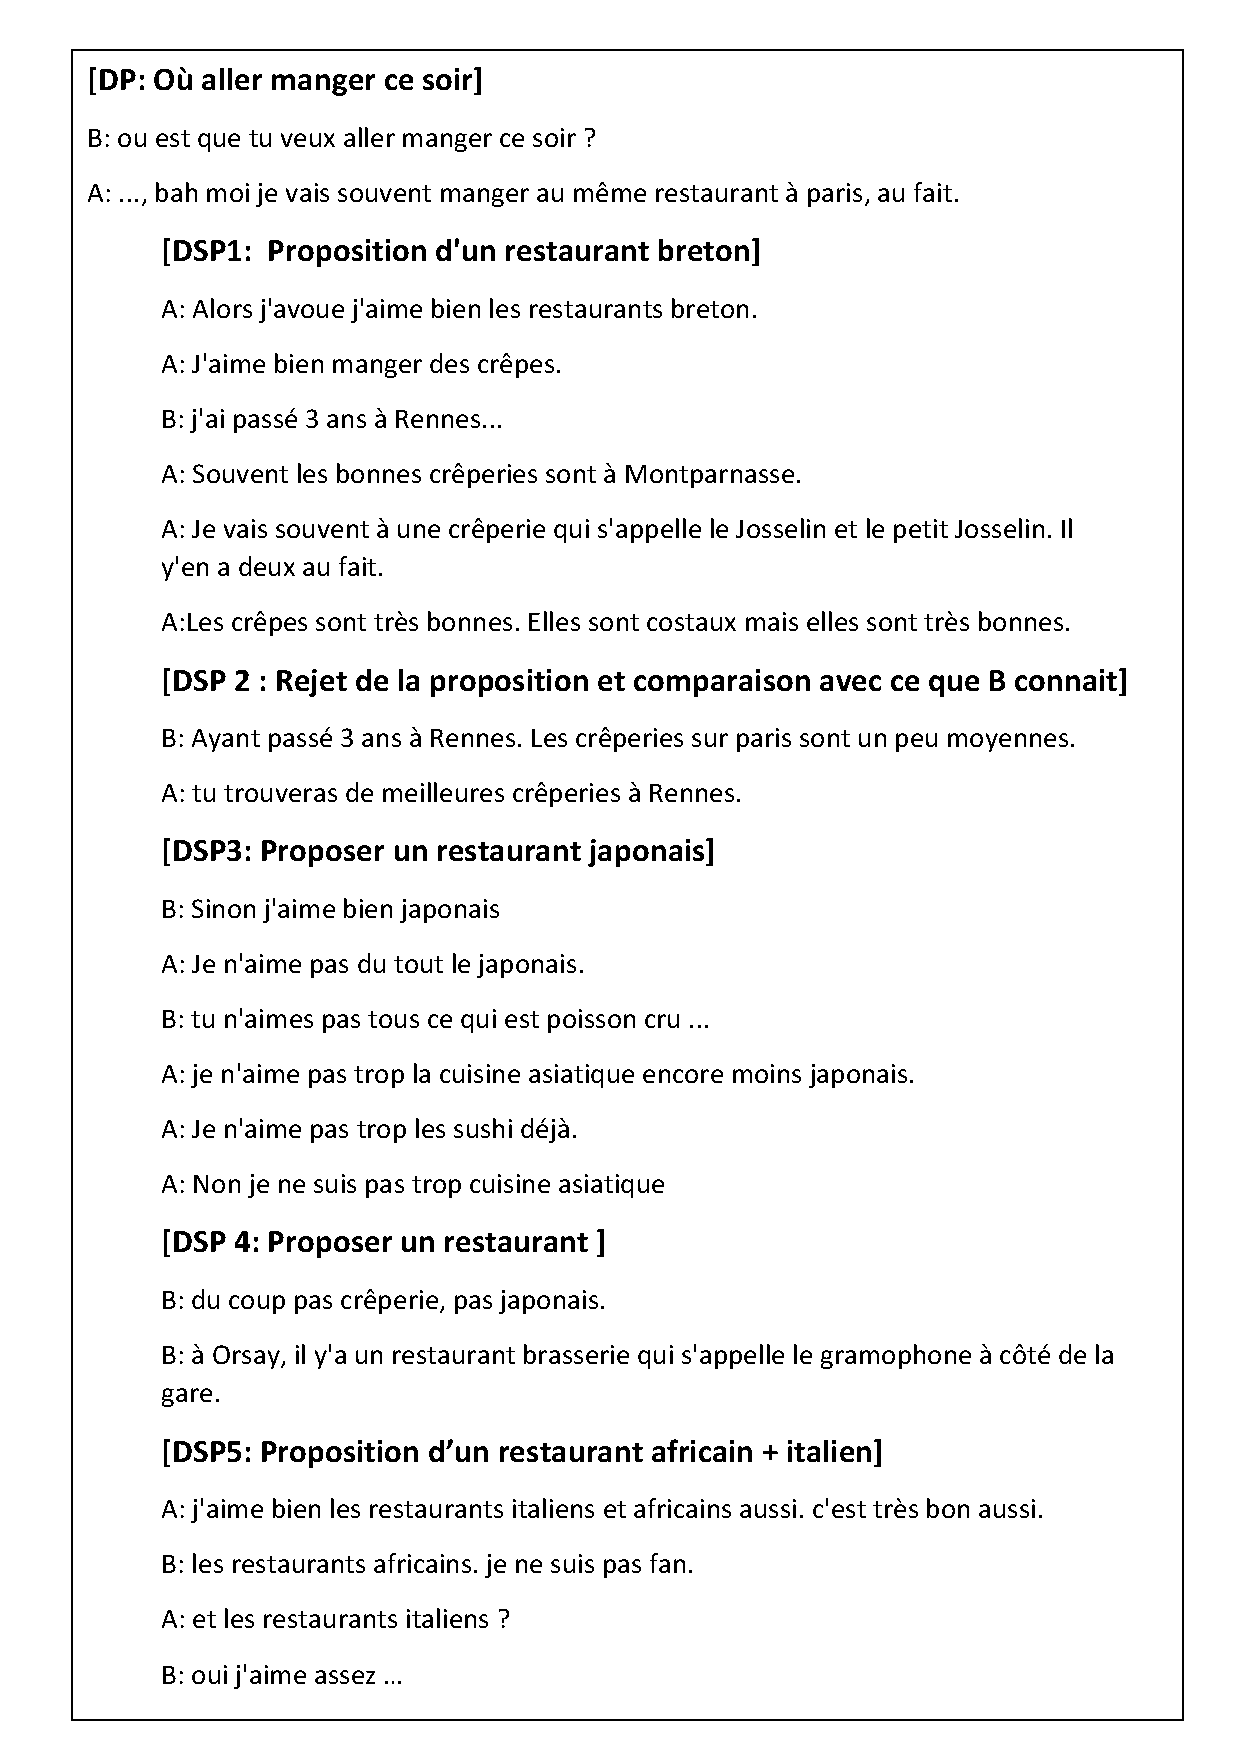
\includegraphics[width=5in]{Figures/dsp_analysis.pdf}
				\caption{\label{fig:conc} Exemple d'une décomposotion en \emph{discourse segment} \emph{DS}}
			\end{figure} 
			 
		\subsection{Résultats de l'analyse}
		
			L'analyse en DSPs nous a révélé un nombre de comportements intéressants tant sur l'aspect structurelle de la négociation que sur les stratégies de négociations déployées par les interlocuteurs. 	
			
			Sur l'aspect structurelle, la décomposition du dialogue en \emph{DS} nous a confirmé que les négociateurs s'intéressaient à différents critères pour le choix d'une option (restaurant dans notre exemple). Ces critères sont négociés simultanément durant la négociation jusqu'a ce que les interlocuteurs trouvent un compromis qui les satisfasse sur les critères jugés importants. 
			Par exemple, dans le premier dialogue, les interlocuteurs se sont plus intéressés à l'ambiance du restaurant et son emplacement pour le choix final. En revanche, dans le second dialogue, les interlocuteurs se sont principalement intéressés aux type et la qualité de la cuisine.
			    
			De plus, Les critères les plus importants sont les premiers à être abordés, et en cas de conflit, d'autre critères sont abordés. 
			Ceci est confirmé par des travaux en négociations automatiques qui mettent en avant l'intérêt de la modalisation multicritères dans les systèmes de négociation. Ce point sera abordé plus en détails en section suivante. 
			 
			 Nous nous sommes aussi intéressé à l'aspect dialogique de la négociation. En effet, notre modèle se basant sur des actes de dialogue, nous avons analysé les différentes informations échangées lors de la négociation. 
			 Nous avons récoltés des informations sur le style linguistique à affecter à nos actes de dialogues.
			 
			 Finalement, nous avons utilisé la structure attentionnelle et intentionnelle afin d'étudier les stratégies de négociation adoptées par les négociateurs. nous avions analyser la corrélation entre différents comportements durant la négociation influencés par la dimension de la dominance.
			 
			 Le résultats obtenus montrent qu'une relation complémentaire de dominance s'installe entre les négociateurs. C'est à dire que dans la situation où un négociateur prend le pouvoir, l'autre parti accepte cette prise de pouvoir et adapte son comportement.
		
			 La prise de pouvoir se manifeste par les stratégies de prise de parole. Le négociateur avec un haut niveau de dominance avait tendance à prendre la parole plus fréquemment, et plus longtemps. Par exemple, en analysant le \emph{DS1} et \emph{DS3}, nous observons que l'interlocuteur \textit{B} prend plus de tours de parole et pour chaque tour, plusieurs actes dialogiques sont énoncés. 
			 %Par conséquent, en moyenne, la
			 
			 
			 De plus, le style linguistique traduit aussi un comportement de dominance, nous avons observé que la personne dominante avait tendance à facilement exprimer ses préférences (\emph{e.g.} voir \emph{DS3}), argumenter ses choix et décisions dans le but de convaincre l'autre. 
			 
			Ces résultats obtenus ont soutenu les comportements de dominance relayé dans les travaux en psychologie sociale et nous ont aidé a orienter la conception de notre modèle de dialogue
			
		
	
	\section{Domaine de négociation}
	\label{domaine}
	
	%	L'interet d'une négociation multi-critères dans la modélisation d'un sujet social
	% voir intro :https://www.ri.cmu.edu/pub_files/pub4/lai_guoming_2008_1/lai_guoming_2008_1.pdf
	%https://link.springer.com/content/pdf/10.1007/s10458-006-9009-y.pdf
	
		La recherche en négociation automatique peut être divisée en deux catégories en ce qui concerne la représentation du domaine: négociation sur un critère et la négociation multi-critères. Cependant, La littérature existante se concentre plus sur la négociation uni critère \cite{lai2008decentralized,lai2004literature}. 
		
		Dans le cadre d'une interaction avec un négociateur humain, la négociation multi-critère est cruciale. En effet, dans un environnement humain, les négociateurs peuvent discuter de plusieurs critères simultanément, ce fait est aussi observé dans l'étude que nous avions effectué dans la section précédente.  Nous avons observé que les négociateurs s'intéressaient à plusieurs critères pour le choix d'un restaurant. Par exemple le type de cuisine, la location ou encore l'ambiance de ce dernier. Ces critères ont soit été abordé simultanément dans la négociation, ou bien un par un. C'est à dire que les négociateurs s'accordaient sur un premier critère avant d'aborder un autre, ou bien discuter des différents critères jusqu'à aboutir a un compromis.
		
		De plus, plusieurs travaux en négociation automatique ont mis en exergue l'apport de la négociation multi-critères. Elle permet d'augmenter la coordination et collaboration durant le processus de négociation afin de rechercher un résultat qui apporte des gains communs pour les deux parties \cite{jonker2007agent,lai2008decentralized,lai2004literature}. \colorbox{red}{Mentionner que la la négociation multicritères  fournit un context permettant voir papier dederu1995 page 3}
	
		% 	Pour toutes ces raisons, notre choix s'est porter sur la négociation multi-critère
	
		Les résultats des précédents travaux nous ont motivé à utiliser une représentation multi-critère pour modéliser notre domaine de négociation collaborative. 
		
		\subsection{Représentation formelle des éléments de la négociation }	
		Le but de la négociation est de choisir une \textit{option} $O$ dans l'ensemble des options $\mathcal{O}$ comprenant toutes les options alternatives envisagé pour un sujet de négociation donnée. 
		
		L'évaluation de chaque option repose sur un ensemble de critères $\mathcal{C}$ reflétant les caractéristiques de l'option. Nous définissons l'ensemble $\mathcal{C}$ de $n$ critères, et $C_1,\ldots,C_n$, comme le domaine de valeurs de chaque critère de l'ensemble. 
		Par conséquent, $\mathcal{O}$ peut être défini comme le produit vectoriel de  $C_1\times\ldots\times C_n$ et chaque option $O \in \mathcal{O}$ est un tuple $(v_1,\ldots,v_n)$. 
		
		Par exemple, une négociation collaborative qui porte sur le choix d'un restaurant où dîner peut être modélisé en prenant en compte quatre critères à savoir $\mathcal{C}$ = \emph{$\{$Cuisine, Prix, Emplacement, Athmosphère, $\}$}. La table \ref{tab:domain} résume un exemple de domaine de valeurs possible pour chaque critère. Nous faisons l'hypothèse que l'agent connaisse toutes les options pour un domaine donné. Un exemple d'option est  \emph{Anterprima(Italien, coûteux , animé, Montparnasse)}. Au total, $638$ options peuvent être généré à partir du domaine présenté dans la table \ref{tab:domain}. 
		\begin{table}[h]
			\centering
			\begin{tabular}{|p{2.25cm}|p{10cm}|}
				\hline
				Critère $i $ & Domaine de valeur $C_i$ \\
				\hline
				Cuisine & \{Italien, Français, Japonais, Chinois, Mexicain, Turque, Coréen\} \\
				\hline
				Atmosphère & \{Animé, Calme, Romantique, Familial, Cosy, Moderne\} \\
				\hline
				Prix & \{Coûteux, abordable, a prix bas\} \\
				\hline
				Emplacement & \{Père Lachaise, Centre de Paris, Montparnasse, Tour Eiffel, gare du Nord\} \\
				\hline
				
			\end{tabular}
			\caption{Domaine de valeurs pour les critères de choix d'un restaurant} 
			\label{tab:domain}
		\end{table}
		
		
		\subsection{Préférences}
		
			L'agent conversationnel est défini avec un ensemble de préférences formalisé  par un ordre partiel $\prec_i$, défini sur chaque domaine de critères $C_i$. 
					\begin{figure}[!tb] 
						\centering 
						\begin{tabular}{l}
							\subfloat[]{\adjustbox{raise=-5pc}{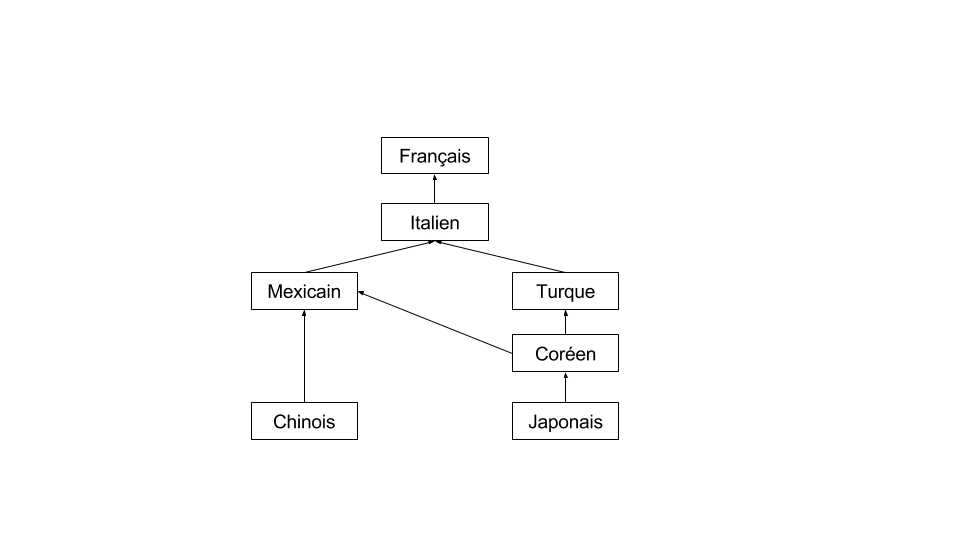
\includegraphics[height=4.8cm]{Figures/cuisine_ex2.png} \label{fig:sub_pref}}}
							\subfloat[]{
								%\input{Figures/Tikz/goldMineState.tex}\label{fig:goldMineState}}  
								\begin{tabular}{|c|c|}
									\hline
									& Critère cuisine \\
									\cline{2-2}
									\parbox[t]{2mm}{\multirow{7}{*}{\rotatebox[origin=c]{90}{\textbf{Préférences}}}} & Japonais $\prec_{cuisine}$ Coréen\\
									\cline{2-2}
									& Chinois $\prec_{cuisine}$ Mexicain\\
									\cline{2-2}
									&  Coréen$\prec_{cuisine}$ Mexicain\\
									\cline{2-2}
									&  Coréen $\prec_{cuisine}$ Turque \\	
									\cline{2-2}
									&  Mexicain$\prec_{cuisine}$ Italien \\
									\cline{2-2}
									&  Turque $\prec_{cuisine}$ Italien\\
									\cline{2-2}
									&  Italien $\prec_{cuisine}$ Français\\	
									\hline								
								\end{tabular}}
							\end{tabular}
							\caption{Exemple de modèle de préférences défini sur le critère cuisine}
							\label{fig:ex_pref}
						\end{figure}
			Nous définissons la relation de préférence comme une relation binaire. Par exemple, $japonais \prec_{cuisine} italien$ signifie que l'agent préfère la cuisine italienne à la cuisine japonaise. Elle est aussi transitive, par exemple, l'agent dispose d'une autre préférence $italien \prec_{cuisine} français$. Nous pouvons donc déduire que l'agent $japonais \prec_{cuisine} français$.
			
			 Ces conditions garantissent que les préférences de l'agent sont cohérentes dans le domaine de la négociation; et la condition de transitivité assure que toutes les valeurs sont comparables. Un exemple de modèle de préférences défini sur le critère de cuisine est présenté dans la figure \ref{fig:ex_pref}.
			
			
			Les préférences étant un aspect essentiel dans la prise de décision durant la négociation, nous avons modélisé une fonction qui représente la valeur d'utilité ou satisfaction pour chaque valeur calculé à partir de l'ensemble des préférences. 
			
			Par conséquent, pour un critère $i\in \mathcal{C}$, pour une valeur $v\in C_i$, l'agent calcule sa \emph{satisfaction} $sat_{self}(v \prec_i)$ pour cette valeur comme le nombre de valeurs qu'il préfère moins dans l'ordre partiel des préférences $\prec_i$. La valeur est ensuite normalisé dans l'intervalle [0,1]:
			
			\begin{equation}
			sat_{self}(v, \prec_i) =	1 - \left( \frac{|\{v' : v' \neq v \  \wedge \ (v \prec_i v')\}| }{( |C_i| - 1 )}\right)
			\end{equation}
			
			La notion de satisfaction est généralisé pour chaque option $o= (v_1, \ldots, v_n)\in \mathcal{O}$ comme une moyenne des valeurs de satisfactions des différentes valeurs de critères: 
			\footnote{Il existe une grande quantité de travaux  dans le domaine de la prise de décision  qui traitent sur la combinaison de plusieurs critères pour le calcul d'utilité en utilisant par exemple des moyennes pondérées ou des intégrales de Choquet. Nous nous ne intéressons pas dans nos travaux à l'optimisation de la fonction de calcul, pour cette raison nous optons pour une fonction simple d'agrégation de préférences.}
	
			\begin{equation}
			sat_{self}(o, \prec) = \frac{\sum_{i=1}^{n} sat_{self}(v_i, \prec_i) }{n}
			\end{equation}
		
			Un exemple de valeurs de satisfactions calculé à partir de l'ensemble des préférences de l'exemple \ref{fig:ex_pref} est illustré dans la table \ref{tab:sat}
					\begin{table}[h]
						\centering
								{\scriptsize
						\begin{tabular}{ |c|c|c|c|c|c|c|c| }
							\hline				
							valeur & Japonais & Coréen & Chinois &  Mexicain & Turque & Italien & Français \\
							\hline
							
							sat(valeur) & 0.16 & 0.33 & 0.5 & 0.66 & 0.66 & 0.83 & 1\\
							\hline
							
						\end{tabular}}
						\caption{Valeurs de satisfiabilité pour le modèle de préférences défini sur le critère de cuisine}
						\label{tab:sat}
					\end{table}
	
	\subsubsection{Communication}
	\label{sec:communication}
		Le modèle de communication est implémenté sur la plateforme \emph{Disco} \cite{rich09}, qui permet à l'agent de communiquer avec l'utilisateur via des actes de dialogues. Chaque acte de dialogue a un ensemble spécifique d'arguments et est associé à une expression spécifique formulé dans un langage naturel (NL).
		
		La modélisation des actes de dialogue est basée sur les travaux de Sidner \cite{sidner1994artificial} qui avait proposé des actes de dialogues qui permettent à un agent de communiquer dans le contexte de négociation collaborative. Ces actes lui permettent aussi de gérer son état mental en terme d'intentions et croyances communiquées durant la négociation. 
		
		Nous avons définis cinq types d'actes de dialogues génériques et deux actes additionnels pour la gestion de fin de négociation. Les actes de dialogues sont présentés dans la table \ref{table:utt}. Seule la génération en langage naturel(LN) de ces énoncés doit être spécifié pour le domaine de négociation. La valeur /$v$/ dans la table \ref{table:utt} fait référence au format en LN pour exprimer une valeur d'un acte de dialogue.
		Nous utiliserons tout le long de ce manuscrit l'exemple d'une négociation collaborative pour le choix d'un restaurant. 
		
		Chaque type d'acte de dialogue prend un argument qui peut être soit un une valeur de critère  $v \in C_i$, une option $o \in \mathcal{O}$ ou encore critère $i \in \mathcal{C}$. 
		
		En fonction des informations qu'ils communiquent, ces actes de dialogues peuvent être divisé en trois groupes:
		
		\begin{enumerate}
			
			\item \textit{Actes de dialogues informatifs}; ce groupe fait référence aux actes de dialogues utilisés pour échanger des informations sur les préférences respectives des négociateurs, à savoir (\textit{AskValue/AskCriterion} et \textit{StateValue}). 
			Nous avons fait le choix d'attribuer une seule valeur pour les actes informatifs car nous avions observé dans les négociations humain/humain enregistrés que les négociateurs utilisaient généralement une formulation pour exprimer les valeurs qu'ils appréciaient ou non. Par exemple \textit{I (don't)like Chinese restaurants} plutôt qu'une expression avec une comparaison binaire du type \textit{I like Chinese more than French}.
			
			\item \textit{Actes de négociation}; ces actes de dialogues permettent à l'agent de gérer la négociation en exprimant des propositions a son interlocuteur (\textit{Propose}) ou bien de répondre à des propositions exprimées par son interlocuteur. L'agent peut accepter ou rejeter une proposition (\textit{Accept, Reject}). Les valeurs en arguments dans les actes de négociation peuvent être soit des valeurs de critère comme (``Let's go to a Chinese restaurant''), soit des options  (``Let's go to \emph{Chez Francis}''). 
			
			\item \textit{Actes de fin de négociation}; les actes  (\textit{NegotiationSuccess} or \textit{NegotiationFailure}) sont utilisés pour clore une négociation soit par une réussite, soit par un échec. Le choix de l'acte dépend de l'état mental de l'agent. En effet, si une option est acceptée par les deux négociateurs, l'agent exprime alors un \textit{NegotiationSuccess} et termine la négociation. Sinon, si la négociation échoue, alors l'agent exprime un \textit{NegotiationFailure}. Les conditions d'échec d'une négociation sont présentées dans le chapitre suivant. 
			
		\end{enumerate}
		 
		
		
			\begin{table}[t]
					\centering
					\begin{tabular} {|p{3.25cm}|p{6cm}|p{3.25cm}|}
						\hline
						\textbf{Type d'acte de dialogue}  &\textbf{ Génération en NL} & \textbf{Postcondition}\\
						\hline
						StateValue(v) &  I (don't) like /$v$/. \newline  J'aime/Je n'aime pas /$v$/ & Speaker : $v \in S_i$ \newline Hearer:  \newline $v\in A_i$ is likable, $v\in U_i$ otherwise \\
						\hline
						AskValue(v)& Do you like /$v$/ ? & \multirow{2}{*}{} \\
						
						AskCriterion(i) &  What kind of /$i$/ do you like ? & \\
						\hline
						ProposeOption(o)  & Let's go to /$o$/. & $o \in P$\\
						
						ProposeValue(v) & Let's go to a /$v$/. & $v \in P_i$\\
						\hline
						AcceptOption(o)& Okay, let's go to /$o$/.& $o \in T$ \\
						
						AcceptValue(v) & Okay, let's go to a /$v$/.& $v \in T_i$ \\
						\hline
						RejectOption(o) & I'd rather choose  something else. & $o \in R$\\
						
						RejectValue(v) &  I'd rather choose  something else. & $v \in R_i$ \\
						\hline
						NegotiationSuccess &  We reached an agreement. & \multirow{2}{*}{}\\
						\cline{1-2}
						NegotiationFailure &  Sorry, but I no longer want to discuss this. & \\
						\hline
						% Counter Propose & $(r,p)\in C_i^2 \vee (r,p) \in \mathcal{O}^2 $ & I don't want to go to $r$. Let's rather go to $p$ \\
						% \hline 
						% RejectState & $x \in \mathcal{O} \vee x\in C_i$ &  I don't like /$x$/, let's choose something else. \\
						% \hline
						% AcceptPropose & $o \in \mathcal{O}$ & Okay. Let's go to /$o$/.\\
						% \hline
					\end{tabular}
				
				\caption{\label{table:utt}Liste des actes de dialogues pour le modèle de négociation collaborative.}
			\end{table}
		
			\subsection{Mise à jour des connaissances durant la communication}
			
			Le choix d'un type d'acte de dialogue est le résultat d'un processus décisionnel que nous détaillerons dans le chapitre \ref{chap:dec}. 
			Afin de prendre des décisions pertinentes, l'agent garde en mémoire l'historique des échanges d'informations formulé au cours de la négociation.  En effet, après chaque acte de dialogue échangé, l'agent met à jour son état mental.  
			
			
			Pour chaque critère $i\in\mathcal{C}$, l'agent construit un ensemble $S_i \subseteq C_i$ des préférences sur les valeurs de ce critère qu'il a déjà communiqué. Cela prévient la répétition d'informations échangées précédemment. 
			De plus, l'agent garde en mémoire les préférences communiquées par son interlocuteur. Nous notons les ensembles $A_i\subseteq C_i$ et $U_i\subseteq C_i$, respectivement l'ensemble des valeurs que l'interlocuteur a communiqué comme appréciées (\textit{I like $\ldots$}) et non appréciées  (\textit{I don't like $\ldots$}) à travers l'acte de dialogue \textit{StatePreference}. 
			
			L'agent maintient aussi des informations sur le cours de la négociation. Soient $P_i \subseteq C_i$, $T_i\subseteq C_i$ et $R_i\subseteq C_i$ les ensembles de toutes les valeurs proposées, acceptées et rejetées pour chaque type de critère. 
			De même, nous considérons $P\subseteq \mathcal{O}$, $T\subseteq \mathcal{O}$ et $R\subseteq \mathcal{O}$ les ensembles de toutes les options proposées, acceptées et rejetées au cours de la négociation.
			
			\subsubsection{Préférences de  l'interlocuteur}
				Dans le contexte d'une négociation collaborative, l'agent prend en compte les préférences de son interlocuteur pour prendre des décision. Pour cette raison, l'agent a besoin de collecter des informations sur les préférences de son interlocuteur. En effet, l'agent utilise les ensembles $A_i$ et $U_i$ qui représentent les préférences de l'interlocuteurs collectés lors des interactions, pour calculer une valeur de \emph{satisfaction}  qu'a l'interlocuteur pour toute valeur $v\in C_i$: 
				
					\begin{equation}
					sat_{other}(v)= \left\{\begin{array}{ll}
					1	 & \mathrm{if\ }  c \in A_i\\
					0    & \mathrm{if\ }c \in U_i\\
					0.5	 & \mathrm{otherwise}
					\end{array}\right.
					\end{equation}
					
				Notons que l'agent possède une connaissance partielle des préférences de son interlocuteur. Par conséquent, les préférences sur certaines valeurs peuvent rester inconnues. Dans  le contexte d'une négociation collaborative, ces valeurs sont considérées comme \textit{potentiellement satisfiables}. Par conséquent, nous leur affectons une valeur arbitraire fixée à \textbf{0.5}.
				
	\section{Conclusion}
			Ce chapitre a présenté les différents éléments de notre modèle de négociation collaborative essentiel pour étudier l'impact de la dominance durant la négociation. Nous avons fait le choix de construire un modèle de négociation générique capable de gérer différent sujets de conversation. De plus, nous avions l'objectifs de définir un domaine qui nous permettrait de refléter différents comportements durant la négociation. 
			
			Premièrement, nous avons appuyé notre recherche par une collecte de données où nous avons enregistré des négociations humains/humain qui nous a révélé nombres de comportements qui apparaissent au cours de la négociation. Ces résultats ont été discutées et nous ont permis de guider notre recherche. Entre autres, les résultats obtenus nous ont soutenu dans notre choix de modéliser une négociation  multi-critères.
			Nous avons donc présenté le domaine de négociation multi-critères ainsi que la représentation classique de préférences.
			
			Nous avons ensuite présenté notre modèle de communication. Le modèle proposé permet à l'agent de mener une négociation collaborative. En effet, les actes proposées permettent à l'agent d'une part d'échanger des informations sur les préférences et d'autre part de négocier. 
			
			Ce modèle de négociation collaborative présente une base solide pour construire un modèle de décision qui prend en compte les comportements de pouvoir. Le chapitre suivant présente donc la construction du modèle décisionnel de notre système de négociation. Nous présenterons un algorithme décisionnel capable de refléter différentes stratégies de négociation en fonction du pouvoir que l'agent cherche à exprimer.
					
			
%	Présentation des actes de dialogues avec leurs catégories et conditions d'applicabilité. 
%	\textcolor{red}{Expliquer que note choix d'utterances se basent sur les travaux de Candece Sidner. De plus, l'analyse en DSP nous a révélé que les participants utiliser des doubles utterances dans leur négociation, et ceci de manière réccurente. Ceci traduisait de plus leur stratégies de négociation influncé par des comportements de pouvoir}
	

%%	
%	\chapter{Modèle de décision basé sur les comportements de pouvoir}
%	\minitoc
%	Après avoir défini la relation interpersonnelle de dominance dans le chapitre \ref{chap:2}, ainsi que sa manifestation dans l'interaction tant sur l'aspect verbal que non verbal, nous avons ensuite détaillé son impact sur les stratégies de négociations. 

Ce chapitre introduit le modèle de décision d'un agent négociateur qui lui permet d'adapter sa stratégie de négociation à la relation de dominance qu'il vise à instaurer avec son interlocuteur. Dans la section 1, nous définissons les principes de décisions basés sur les comportements de pouvoir inspirés des travaux en psychologie sociale. Dans la section 2, nous présentons un premier modèle décisionnel utilisant des règles de décisions.  Pour ce modèle, nous nous sommes basés sur la structure d'arbres défini dans \emph{DISCO} \cite{ri} et nous discuterons ses limites. Ensuite dans la section 3, nous présenterons notre modèle décisionnel final qui prends en compte les comportements de pouvoir de l'agent associés à ses préférences pour construire sa stratégie de négociation. Ensuite, nous présenterons deux études visant à valider le modèle décisionnel dans les deux cas d'interaction agent/agent et agent/humain.

\section{Comportements de pouvoir et stratégies de négociation}

 Comme nous l'avons présenté dans le chapitre \ref{chap:2}, nous nous sommes essentiellement basés sur les travaux en psychologie sociale pour la définition de la dominance. 
 La dominance comme relation interpersonnelle est présentée comme la capacité à exprimer des comportements de pouvoir où l'influence est atteinte. Prenant cette définition comme point de départ, nous nous sommes ensuite intéressé à la manifestation des comportements de pouvoir durant le processus de négociation et comment ces comportements influencé les stratégies de négociations dans le contexte d'interaction humain/humain. 
 
 Dans ce qui suit, nous présentons \emph{trois principes} de comportements extraits des travaux en psychologie sociale qui ont étudiaient l'impact du pouvoir sur les négociateurs et leur stratégies.
 
	\begin{enumerate}
	\item \textbf{Niveau d'exigence et de concessions:} Les négociateurs avec un pouvoir élevé affichent un niveau d'exigence plus important comparés aux négociateurs avec un pouvoir plus faible. Par ailleurs, les exigences des négociateurs de faible pouvoir diminuent avec le temps. Ceci se traduit par des concessions plus importantes comparés aux négociateurs avec un pouvoir plus important. \cite{de1995impact}
	
	\item \textbf{Soi \emph{vs} autrui:} Les négociateurs de faible pouvoir prennent en compte les préférences de leur interlocuteur dans la négociation, tandis que les négociateurs avec un pouvoir plus grand sont  centrés sur eux-mêmes et s'intéressent uniquement à la satisfaction leurs propres préférences. \cite{fiske1993controlling,de1995impact}
	
	\item \textbf{Contrôle du flux de la négociation:}
	Les négociateurs avec un pouvoir élevé ont tendance à faire le premier pas et à prendre les devants dans la négociation \cite {magee2007power}. Ils sont centrés sur l'avancement du processus de prise de décision, en prenant des décisions rapides \cite{zablotskaya2012relating}.
	  A l'opposé, les négociateurs de faible pouvoir visent à construire un modèle précis des préférences du partenaire de négociation. 
	  Par conséquent,  ils posent plus de questions afin de collecter les informations nécessaires qui leurs permet de prendre la décision la plus équitable(\emph{e.g}  faire des propositions)~\cite{de2004influence}. 
	
\end{enumerate}


Le but est de construire un modèle de décision capable d'illustrer ces comportements de pouvoir et par conséquent, adapter la stratégie de négociation en fonction du pouvoir que l'agent veut exprimer.

Dans ce qui suit nous présenterons, le modèle décision de l'agent qui prend en compte la relation de pouvoir.

 
\section{Règles de décision}
	Nous avons construit des règles de décision modélisées sous forme d'arbres de dialogues. L'implémentation de notre système de dialogue étant géré par le logiciel \emph{DISCO}. Disco est une implémentation d'un ``collaborative discourse manager'' inspiré d'une théorie de dialogue collaboratif comme Collagen \cite{rich1997collagen}. Disco est un système qui permet la génération de dialogues orienté tâches pour lequel il utilise le formalisme des HTNs (Hierarchical Task Networks) \cite{erol1994htn} pour la gestion des tâches. Il est implémenté avec le standard ANSI/CEA-2018 : chaque tâche est définit avec des préconditions, des effets et des postconditions. Les tâches sont regroupées par \emph{recettes} munies de conditions d'applicabilité.
	
	De plus, Disco a été étendu avec un module génération d'arbres de dialogues afin de communiquer et collaborer avec l'utilisateur pour la réalisation des tâches. Ce module est nommé Disco for Games (D4g) et permet de définir des sémantiques d'actes de dialogue. D4g est déjà fourni avec un ensemble d'actes de dialogue.
	
	Nous avons complété ce système avec les actes de dialogues présenté dans la section \label{sec:communication} afin qu'il puisse supporter la négociation sur les préférences.
	
	Pour chaque acte de dialogue que l'agent reçois, nous modélisons l'ensemble des réponses que l'agent peut sélectionner. Par exemple, suite à un acte \emph{Propose} énoncé par l'utilisateur, l'agent peut répondre par un \emph{Accept}, un \emph{Reject} ou un autre \emph{Propose} ("User: Allons au Chinois. Agent: Et si nous allions plutôt au Japonais?"). 
	Chaque branche est définie avec des conditions d'applicabilités pour décider quelle réponse est adoptée. 
	Ces conditions prennent en compte le pouvoir de l'agent en plus du contexte courent de la négociation. Dans l'exemple précédent, l'agent doit être dominant pour répondre à un Propose par un autre Propose. 
	
	

	
	\subsection{Sélection de l'acte de dialogue}
		Nous avons initialisé l'agent avec un comportement de pouvoir parmi trois types de comportements de pouvoir inspirés de la littérature en psychologies social.  L'agent peut suivre un comportement \emph{dominant, soumis} ou \emph{neutre}. 
		
		En fonction de l'acte de dialogue que l'agent reçoit, nous générons un ensemble de réponses possibles. Chaque réponse dépend du pouvoir de l'agent. Le système de dialogue offre à l'utilisateur la liberté de choisir n'importe quel acte de dialogue pour son tour de parole. Disco déroule alors l'arbre de dialogue correspondant de gauche à droite (en commençant par la branche la plus à gauche). La première branche applicable rencontrée est directement exécutée sans vérifier les branches restantes.
		
		Notons que dans la suite, chaque arbre de dialogue est défini avec une condition de sortie qui clos la négociation avec un échec. Cette dernière est activée seulement par agent \emph{dominant} dans la situation où toutes les valeurs restantes ne sont pas acceptables. 
		
		\subsubsection{AskPreference}
	
	
		\subsubsection{State Preference}
			Le comportement standard qu'un agent adopte à la réception d'un \emph{StatePreference(v)} est de donner son opinion sur la valeur exprimée (c-à-d que l'agent calcule la valeur de satisfiabilité de \textit{v}). Cependant, si l'agent a déjà exprimé ses préférences sur ces valeurs, il va vouloir choisir un autre acte de dialogue en fonction de la relation sociale:
			\begin{itemize}
				\item \emph{Propose(x)}: Si l'agent est \emph{soumis} ou si il a la même préférence que l'utilisateur, il va proposer de choisir la valeur préférée de l'utilisateur.
				\item \emph{Propose}: Si le nombre de \emph{StatePreferences} autorisé est atteint (voir figure \ref{alg:maxtours}), l'agent doit respecter le principe 3 et faire évoluer la négociation. La valeur proposé doit respecter les préférences de l'agent. 
				\item \emph{StatePreference}:l'agent est \emph{soumis} ou \emph{neutre}, il va vouloir exprimer ses préférences afin de construire une meilleure connaissance.
				\item \emph{AskPreference}:l'agent est \emph{neutre} ou \emph{dominant}. Dans le cas où toutes les valeurs du critères courent ont été discutés, l'agent va respecter le principe 3 et faire évoluer la négociation en ouvrant la discussion sur un autre critère.
			\end{itemize}
			
			\begin{figure}[]
				\begin{algorithmic}[1]\small
					\Function{MaxStatements}{}
					\State $nbTours$ = Nombre de \emph{StatePreferences} exprimés successivement.
					\State $maxTours$ 
					\If{($dominant$)} 
					\State $maxTours = 1$
					\EndIf
					\If{($peer$)} \State $maxTours = 2$
					\EndIf
					\If{($soumis$)} 
					\State $maxTours = 4$
					\EndIf
					\State $retrun$ $nbTours\geq maxTours$
					\EndFunction
				\end{algorithmic}
				\vskip 8pt
				\label{alg:maxtours}
				\caption{Maximum de tours de \emph{StatePreference} autorisé en fonction du pouvoir de l'agent}
			\end{figure} 
		\subsubsection{Propose}
			A la réception d'un \emph{Propose} comme présenté dans la figure ..., l'agent choisit sa réponse en fonction de l'\emph{acceptabilité} de la proposition.
			Nous avons écrit l'algorithme d'acceptabilité afin qu'il s'adapte à la valeur de pouvoir de l'agent. Ce choix permet de refléter les comportements du principe 2 \emph{niveau d'exigences et concessions}.
			
			En effet, au fur et a mesure que la négociation évolue, l'agent décide de faire des concessions sur certains critères. Par exemple, il peut considérer que le critère de \emph{localisation} n'est plus important pour le choix d'un restaurant. Par conséquent, il considérera que toute valeur de \emph{localisation} est désormais \emph{acceptable}.
			
			Par ailleurs, la notion d'exigence apparaît dans l'algorithme ci-dessous. Si l'agent est \emph{dominant}, l'ensemble de valeurs acceptables est plus restreint qu'un agent \emph{soumis}.
			
			\begin{figure}[]
				\begin{algorithmic}[1]\small
					\Function{isAcceptable}{$proposal$}
					\If{(type de $proposal$ n'est pas un critère important)} 
					\State return $true$
					\EndIf
					
					\State List = trier les valeurs par ordre décroissant de préférences
					\If{($dominant$)} 
					\State $return$ index($proposal$)< $size(List)/2$
					\EndIf
					\If{($soumis$)} 
					\State return $return$ index($proposal$)< $size(List)/4$
					\EndIf
					\EndFunction
				\end{algorithmic}
				\vskip 8pt
				\label{pseudo}
				\caption{Calcul d'acceptabilité d'une proposition $value$}
			\end{figure} 
			
			
			L'arbre de décision produit pour répondre à un \emph{Propose(p)} est présenté dans la figure .... 
			\begin{itemize}
			
				\item  \emph{Accept(p)}: Si la proposition $p$ est acceptable, l'agent doit exprimer un \emph{Accept(p)}. Sinon, l'agent doit faire évoluer la négociation pour trouver un meilleurs compromis. En fonction de la relation de pouvoir l'agent choisit un acte de dialogue spécifique.
				\item \emph{Ask :} l'agent \emph{soumis} va suivre les comportements décrit dans les principes 1 et 3. En effet, il va essayer de collecter plus de connaissances sur les préférences de l'autre et ainsi prendre en compte ses préférences. 
				\item \emph{Reject :} l'agent qui n'est pas dominant (\emph{i.e. soumis ou neutre}) rejete une proposition qui n'est pas acceptable.
				\item \emph{Propose :} suivant le principe 3, l'agent \emph{dominant} fait évoluer la négociation en proposant une autre valeur qui respecte mieux ses préférences. 
			\end{itemize}
	
			 
	
		\subsubsection{Accept }
			A la réception	d'un \emph{Accept}, nous séparons deux cas de réponses en fonction du type de la valeur acceptée $v$.
			Premièrement, $ v \in \mathcal{O}$ une \textit{option}, l'agent clos la négociation par un \emph{succès}.
			Sinon, $v \in C_i$ est une valeur de critère, l'agent entame la négociation sur un autre critère et sa réponse sera choisie en fonction de la relation de pouvoir à exprimer.
			
			\begin{itemize}
				\item \emph{Propose}: La condition d'applicabilité pour cet acte de dialogue dépend du pouvoir de l'agent. Un agent \emph{dominant} entamera la négociation sur le nouveau critère en proposant une valeur qui respecte ses préférences. Cependant, un agent \emph{soumis} n'est autorisé à faire une proposition que s'il a des connaissances sur les préférences de l'autres,  communiqués par des \emph{StatePreferences}, qui lui permettront de prendre une décision équitable. cet algorithme traduit les comportements présentés dans les principes 1 et 3. 
				
				\item \emph{AskPreference}: Comme présenté dans le principe 3,l'agent est \emph{soumis} collecte le plus d'informations possibles sur les préférences de son interlocuteur. 
				\item \emph{StatePreference}: L'agent est \emph{peer} ouvre la négociation en communiquant ses préférences sur le nouveau critère à discuter. 
				
			\end{itemize}
			
%				\begin{figure}[]
%					\begin{algorithmic}[1]\small
%						\Function{CanPropose}{}
%						\If{($dominant$)} 
%						\State return $true$
%						\EndIf
%						
%						\State 
%						\If{($soumis$)} 
%						\State l'agent a des connaissances suffisantes sur les préférences de l'interlocuteur
%						\State return $true$
%						\EndIf
%						\EndFunction
%					\end{algorithmic}
%					\vskip 8pt
%					\label{alg:canPropose}
%					\caption{Calcul d'acceptabilité d'une proposition $value$}
%				\end{figure}
%				
				
		\subsubsection{Reject}
			Suite à un \emph{Reject}, l'agent choisis une réponse en suivant les trois principes comme présenté ci-dessous:
			\begin{itemize}
				\item \emph{AskPreference}: Si la proposition d'un agent \emph{soumis} est rejetée, il va considérer qu'il n'avait pas assez de connaissances pour prendre une bonne décision. Pour compenser, il va demander à l'utilisateur ses préférences sur des valeurs qu'il ne connaît pas déjà. 
				
				\item \emph{Propose}: Suivant les principes 1 et 3, l'agent \emph{dominant} fait avancer la négociation en proposant de nouvelles valeurs. Cependant, si la valeur rejetée se trouve être la valeur qu'il préfère le plus, il va refuser de concéder et donc proposer la valeur encore une fois. Ce comportement est fidèle au principe 2. 
				
				\item \emph{StatePreference}: l'agent \emph{peer} continue la négociation en exprimant ses préférences sur d'autres valeurs. 
			\end{itemize}	
		%----------------------------------------------------------------
			
	\subsubsection{Exemple}	Exemple de fdialogue généré
	
	\subsection{Limites des arbres de dialogue}
		Parler de l'étude qui a montré une ambiguité dans la perception des comportement et la capacité à isoler l'impact de chaque principe sur la prise de décision
		
		Comportement incongrue ou non attendue.
		
		Situation de \textit{breakdown}, du a une modèlisation manuelle, nous avions rencontrer des situations où aucune condition d'applicabilité n'étaient vrai. 
		
		Pour toutes ces raisons, nous avons repenser notre solution pour qu'elle soit plus fidèle aux principe de négociation et qu'elle puisse refléter les comportements de pouvoir. 
	
	\section{Modèle de décision basé sur les comportements de pouvoirs}
	
%\chapter{Complémentarité Vs Similarité dans la relation de dominance}
%
%%	\minitoc
%	\chapter[Complémentarité Vs Similarité]{Complémentarité Vs Similarité dans la relation de dominance}
\label{chap:chap6}
	\begingroup
	\parindent=0em
	\etocsettocstyle{\rule{\linewidth}{\tocrulewidth}\vskip1\baselineskip}{\rule{\linewidth}{\tocrulewidth}}
	\emph{\textbf{Sommaire}} \vspace{0.5em}
	\localtableofcontents 
	\clearpage
	\endgroup
Dans ce chapitre, nous présenterons une autre étude de l'interaction entre un utilisateur et un agent virtuel dans le contexte d'une négociation collaborative. 
Notre objectif est d'étudier l'influence de la relation interpersonnelle de dominance sur le processus de négociation. 

En premier lieu, les objectifs généraux de cette étude seront présentés (section \ref{sec:obj}). Nous détaillerons la méthodologie employée pour le paramétrage des agents utilisés dans cette expérimentation (section \ref{sec:methodo}) ainsi que les hypothèses que nous formulons (section \ref{sec:H}).

Nous présenterons ensuite le protocole expérimental employé (section \ref{sec:procedure}). Enfin, nous décrirons les résultats obtenus  (section \ref{sec:res})
que nous discuterons ensuite \ref{sec:discussion}
\section{Objectif}
\label{sec:obj}

Plusieurs études en psychologie sociale ont exploré l'impact de la relation de dominance sur l'expérience de la négociation et de ses résultats. Certains travaux ont montré que l'expression de comportements complémentaires de dominance permettait d'améliorer la coordination et donc le gain commun des négociateurs. En conséquence, les négociateurs se sentaient plus à l'aise. \cite{tiedens2003power,wiltermuth2009benefits,olekalns2013dyadic}.
En parallèle, d'autres travaux ont étudié l'impact de la similarité dans les comportements de dominance dans la négociation. Ces derniers suggèrent que la similarité dans les comportements non verbaux de dominance améliore l'interaction et le processus de négociation car les individus sont attirés par ceux qui expriment des comportements similaires. Ceci permet d'augmenter le sentiment d'affiliation \cite{olekalns2013dyadic}. 

En vue des contradictions dans la littérature sur l'impact de la complémentarité et la similarité des comportements de dominance dans les interactions, des chercheurs ont mené des études pour comparer les deux approches et étudier laquelle permettait d'avoir de meilleures influences sur l'interaction \cite{tiedens2003power,dryer1997opposites}. Ces études ont montré que la complémentarité de dominance dans les comportements non verbaux s'installait de manière inconsciente entre les individus. De plus, les participants ont préféré interagir avec les individus qui adoptaient un comportement complémentaire et se sentaient plus à l'aise comparés avec ceux qui exhibaient des comportements similaires. 


Partant de ces études, notre objectif est d'explorer l'impact de ces comportements de dominance qu'ils soient complémentaires ou similaires sur les stratégies de négociation dans le contexte d'une négociation collaborative entre un agent et un utilisateur. Cependant, comme la relation de dominance qui s'installe durant l'interaction est forcément complémentaire nous pensons que les stratégies complémentaires auront un impact positif plus important que des stratégies similaires.

\subsection{Complémentarité en psychologie sociale}
	Nous avons présenté dans la section \ref{sec:compEtat} la littérature sur les comportements complémentaires de dominance dans la négociation. Nous rappelons dans cette sections les principaux résultats: 
	
	\begin{itemize}
		\item La complémentarité dans les comportements de dominance améliore la coordination entre les négociateurs qui a pour résultat d'améliore le gain commun des négociateurs.
		
		\item La création de valeurs durant la négociation est plus importante dans des dyades où les négociateurs affichent des comportements complémentaires de dominance
		
		\item En conséquence, le sentiment de confort est accru dans les dyades complémentaires comparées aux dyades similaires. De plus, la complémentarité permet d'améliorer l'appréciation entre les négociateurs.
	\end{itemize}
	

Nous présentons dans la suite de ce chapitre notre étude qui vise à analyser ces comportements dans le contexte d'une négociation entre un agent et un utilisateur humain.

\section{Méthodologie}
\label{sec:methodo}

Afin d'illustrer notre modèle de négociation, nous reprenons le scénario d'une négociation collaborative pour le choix d'un restaurant.
Ce scénario ne nécessite aucune une expertise pour prendre part dans la négociation. De plus, il est facile pour les participants de reporter leurs préférences pour les différents critères pris en compte pour le choix d'un restaurant. En effet, nous considérons le même sujet de négociation des restaurant avec les mêmes critères. Nous avons enrichis le domaine de valeurs des critères. Chaque critère est défini avec un ensemble de valeurs présenté dans la table \ref{tab:valeursCritere}. Un total de 630 restaurants ont été générés à partir des critères regroupant les différentes possibilités.

\begin{table}[b]
	\caption{Ensemble de valeurs possible pour chaque critère afin de choisir un restaurant}
	\label{tab:valeursCritere}
	\centering
	\begin{tabular}{ >{\centering\arraybackslash}m{2cm}| >{\centering\arraybackslash}m{9cm}}
		\hline
		\hline
		\textbf{Critère} & \textbf{Ensemble des valeurs} \\
		\hline
		Cuisine & Chinois ,Français ,Italien ,Japonais ,Coréen ,Mexicain ,Turc \\
		\hline
		Ambiance & cosy ,familial ,anime ,moderne ,romantique ,calme \\
		\hline 
		Prix  & abordable ,bas prix ,chic \\
		\hline
		Localisation & centre de paris ,Gare du nord , Montparnasse , près de la tour Eiffel ,Père lachaise \\
		\hline
		\hline
	\end{tabular}
\end{table}

Trois paramètres importants sont à prendre en compte pour initialiser les comportements des agents. 
En premier lieu, il faut fixer la valeur initiale de dominance affectée à chaque agent. Nous avons choisi une valeur de dominance $dom =0.55$ afin de générer des comportements de dominance initialement neutres.

En second lieu, il faut initialiser les préférences des agents. Afin de placer les sujets dans des conditions comparables quelles que soient leurs préférences, nous avons demandé aux participants de saisir leurs préférences (voir section \ref{sec:procedure}).

A partir des préférences saisies par le participant, nous générons automatiquement les préférences des agents suivant certaines conditions.
La première condition visait à générer des modèles de préférences différents de celui communiqué par l'utilisateur dans le but de créer une confrontation qui pousse à la négociation. Pour cela, nous avons utilisé la distance de kendall \cite{bra2013Kendall}  (\emph{Kendall's  $ \tau \in [0,1]$}) afin de définir la limite minimale de différence entre le modèle de l'agent et celui de l'utilisateur. Par conséquent, nous avons fixé la distance à (\emph{Kendall's  $ \tau \geq 0.7$}).

La seconde condition assurait la différence entre les modèles de préférences générées pour les différents agents qui vont interagir avec les sujets. 
Notre objectif est d'éviter une forte ressemblance entre les préférences des agents qui donnerait l'impression d'interagir avec la même entité.

Nous avons donc gardé uniquement des modèles différents (Kendall's  $ \tau \geq 0.35$). De plus, nous avons ajouté une condition qui assure une différence de perception: pour chaque critère, les modèles devaient avoir des valeurs différentes pour représenter la valeur la plus préférée de l'agent. 
Cela permet de renforcer le sentiment d'interagir avec un agent différent, la valeur préférée étant souvent la première à être proposée par l'agent. 
%Par exemple, considérons deux modèles \emph{P1, P2} générés et qui ont une distance est supérieur à $0.35$. De plus, pour le critère \textit{cuisine}, les deux modèles ont la valeur $Italien$ comme la valeur la plus satisfiable $sat_{P1}(Italien) = 1$ et $sat_{P2}(Italien) = 1$. Ces deux modèles sont automatiquement rejetés.

En dernier lieu, nous avons paramétré la stratégie comportementale des agents. Comme notre but est d'analyser l'impact de la complémentarité ou de la similarité de la dominance durant la négociation, nous avons implémenté trois stratégies distinctes reproduisant les comportements désirés. 
A partir de notre algorithme de la théorie de l'esprit présenté dans le chapitre \ref{chap:Tom}, l'agent calcule la valeur de dominance de l'utilisateur $dom_{user}$ pour chaque tour de parole exprimé par ce dernier. Suivant la valeur de dominance calculée $dom_{user}$, l'agent adopte une des stratégies suivantes:


%	Nous avons implémenté trois agents, tous initialisé avec une valeur de dominance
%	De plus, chaque agent adopte une stratégie distincte représentant une condition expérimentale pour notre étude: 

\begin{enumerate}
	\item \textit{Comportement complémentaire}: A chaque tour de parole, l'agent révise sa valeur de dominance pour qu'elle soit complémentaire à celle détéctée pour son partenaire $dom_{agent}=1-dom_{user}$.
	
	\item \textit{Comportement similaire}: L'agent va imiter les comportements de dominance exprimées par le participant $dom_{agent} = dom_{user}$.
	
	\item \textit{Comportement neutre} : L'agent ne s'adapte pas à son interlocuteur et suit un comportement de dominance statique.
	
	 $dom_{agent} = dom_{agent} (t=0)$
\end{enumerate}

En modifiant la valeur de dominance de l'agent à chaque tour, nous avons dû ajouter une contrainte dans son modèle décisionnel afin d'assurer une cohérence dans les comportements générés. 
En effet, la valeur de dominance est essentielle pour le calcul des satisfiabilités des valeurs et un changement de cette valeur risque de fausser l'ordre des valeurs satisfiables de l'agent.
Par exemple, à un moment $t$ de la négociation, une valeur $v$ est satisfiable, mais due à une adaptation qui cause un changement de dominance la même valeur $v$ peut devenir non satisfiable. Par conséquent, l'agent peut dire à un tour aimer une valeur et aux tours suivant refuser une proposition pour cette même valeur.

En vue de protéger des préférences et donc la cohérence des comportements de l'agent, nous avons fait le choix d'utiliser uniquement la valeur de dominance initiale $dom_{agent} = 0.55$ pour calculer la satisfiabilité des valeurs.

Nous avons donc implémenté trois agents \emph{Bob, Arthur} et \emph{Kevin}. \emph{Bob} adoptant un comportement complémentaire, \emph{Arthur} qui suit un comportement similaire à celui exprimé par son partenaire de négociation, et enfin \emph{Kevin}, un agent contrôle qui suit une seule stratégie de dominance neutre. 

\section{Hypothèses}
\label{sec:H}

Suivant les travaux de \cite{tiedens2003power,dryer1997opposites,wiltermuth2015benefits}, nous supposons que la relation de dominance établie entre l'agent et l'utilisateur a une influence sur les stratégies exprimées par les négociateurs. Elle va donc avoir une conséquence sur les résultats obtenues lors de la négociation ainsi que le niveau d'appréciation à négocier avec l'agent.
Nous faisons les hypothèses suivantes: 
\begin{itemize}
	\item [$\bullet$] \textbf{H1}: Les comportements de complémentarité et de similarité des agents virtuels sont perçus par les participants.
	\item [$\bullet$] \textbf{H2}: Les négociateurs atteignent un gain commun plus important quand les négociateurs établissent une relation de dominance complémentaire.
	\item [$\bullet$] \textbf{H3}: La négociation converge plus rapidement dans le cas où les négociateurs ont une relation de dominance complémentaire. 
	\item [$\bullet$] \textbf{H4}: Le négociateur se sent plus à l'aise avec un partenaire qui exprime un comportement complémentaire.
	\item [$\bullet$] \textbf{H5}: La complémentarité dans la relation de dominance augmente l'appréciation entre les négociateurs.
\end{itemize}



\section{Protocole expérimentale}
\label{sec:procedure}
Nous présentons dans cette section, le protocole expérimental employé, en commençant par les mesures utilisées pour questionner les participants sur leurs interactions avec les différents agents. Ensuite, nous présenterons la population de participants et enfin le protocole suivi pour chaque participant. 

\subsection{Mesures}
Après chaque interaction avec un agent, le participant était invité à remplir un questionnaire sur la perception des comportements de dominance.
Nous avons repris les trois principes de dominance (voir section \ref{chap:domer}) pour évaluer les comportements des participants et des agents. De plus, pour chaque questionnaire, nous avons insérés quelques items de manipulation afin de vérifier la concordance des réponses.  Les trois principes représentent quatre comportements de dominance, à savoir :
	\begin{itemize}
		\item \textbf{D1}: La prise en compte des préférences de l'autre dans la prise de décision. Nous avons évalué l'égocentrisme des négociateurs dans leurs stratégies de négociation. 
		\item \textbf{D2}: Le niveau de concessions exprimé durant la négociation.
		\item \textbf{D3}: Le niveau d'exigence du négociateur.
		\item \textbf{D4}: Le négociateur est leader dans la négociation.
	\end{itemize}

\subsubsection{Questionnaire en auto-attribution} Les participants ont répondu pour eux-mêmes au questionnaire des comportements de dominance dans la négociation que nous avons conçu, afin de mesurer les comportements qu'ils ont exhibé durant leur interaction. Ce questionnaire utilise une échelle de Likert à 5 points. Nous présentons ci-dessous les items de ce questionnaire. 
\begin{enumerate}
	\item J'ai été égocentrique pendant la négociation
	\item J'ai pris en compte les préférences de l'agent.
	\item J'ai été exigeant(e).
	\item J'ai maintenu ma position durant la négociation.
	\item J'ai abandonné ma position durant la négociation
	\item J'ai fait des concessions pendant la négociation.	
	\item J'ai mené la négociation.
	\item J'étais leader dans la négociation
\end{enumerate}

\subsubsection{Questionnaire en hétéro-attribution}
Les participants ont répondu à un questionnaire afin de décrire leur perception de l’agent avec lequel ils interagissaient.

Nous nous sommes principalement intéressés aux comportements de dominance exprimée par l'agent. Pour cela, nous avons utilisé le même questionnaire sur les comportements de dominance (voir section \ref{sec:questionnaire})

\subsection{Questionnaire concernant l'interaction}
Pour évaluer l'appréciation du participant vis à vis de l'interaction qu'il a eu avec l'agent. Nous nous sommes basés sur les travaux de \cite{tiedens2003power,wiltermuth2009benefits,olekalns2013dyadic} pour définir le questionnaire ci-dessous:

\begin{enumerate}
	\item Je suis satisfait de la décision finale.
	\item La décision finale était équitable pour nous deux.
	\item Je me suis senti à l'aise pendant la négociation.
	\item J'ai trouvé que la négociation avec l'agent était aisée.
	\item Je me sentais détendu pendant la négociation.
	\item Je me sentais anxieux pendant la négociation.
	\item J'ai apprécié la négociation avec l'agent.
\end{enumerate}

\subsection{Données d'interactions}
Nous avons enregistré les informations suivantes à chaque interaction
\begin{itemize}
	\item Les préférences du participant et celles de l'agent.
	\item Le nombre de tours de négociation avant de trouver un compromis
	\item La position du participant dans le spectre de dominance calculé à partir de l'algorithme de théorie de l'esprit après chaque tour de parole.
	\item Le dialogue généré.
	
\end{itemize}


\subsection{Protocole}
Après avoir expliqué le but de l'étude qui portait sur l'évaluation des comportements d'agents virtuels, l'expérimentateur développait le déroulé de l'étude. 
Premièrement, il expliquait que le but de l'interaction était de négocier avec chaque agent afin de trouver un restaurant où aller dîner. Il leur donnait des instructions afin de se projeter dans une situation réelle en plus de mettre l'accent sur l'aspect "collaboratif" de la négociation comme présenté dans la figure \ref{fig:instruction}.

\begin{figure}[h]
	\fbox{\begin{minipage}{.95\textwidth}
			{\ttfamily
				\textbf{Instruction:} Mettez vous dans la situation où vous allez dîner avec un ami ou un collègue pour la première fois, vous ne connaissez pas ses goûts et il ne connaît pas les vôtres. Le but est de négocier en fonction de vos préférences respectives pour de choisir un restaurant qui \underline{vous convienne à tous les deux}.
			}
		\end{minipage}}
		
		\caption{\label{fig:instruction}Explication du but de l'étude.}
	\end{figure}
	
	
	Une fois le but de l'étude expliqué, l'expérimentateur lançait la phase de tutoriel afin de familiariser le participant à l'utilisation de l'interface de communication. L'expérimentateur présentait les différents les actes de dialogues possibles pour communiquer avec l'agent. 	
	Le participant était informé que durant cette session l'agent ne répondait pas à ses actes, et que le but était uniquement de manipuler l'interface pour générer des actes. 
	
	L’expérimentateur répondait alors à d’éventuelles questions concernant la génération d'actes de dialogue ou leurs significations.
	
	Ensuite, l’expérimentateur annonçait au participant qu’il/elle allait négocier avec trois  agents virtuels différents et
	qu’après chaque négociation, il/elle devrait répondre à différents questionnaires pour évaluer son interaction avec l’agent avec lequel il/elle venait de négocier.  Avant de commencer l'expérience, le participant est invité à saisir ses préférences pour les valeurs de chaque critère (voir la figure \ref{fig:pref}).
	
	Une fois les préférences pour les différentes valeurs de critères saisies, la fenêtre avec le premier agent s'ouvrait automatiquement invitant le participant à prendre part à la négociation. 
	
	\begin{figure}[b]
		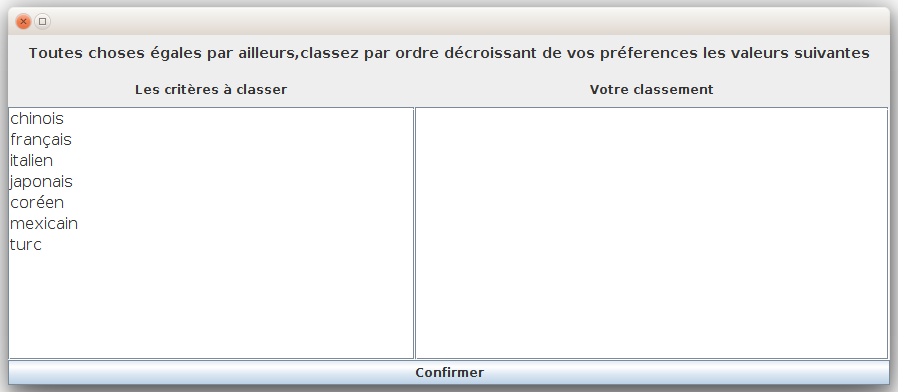
\includegraphics[width=4in]{Figures/pref.png}
		\caption{\label{fig:pref} Interface pour la saisie d'ordre de préférence. Exemple pour le critère de cuisine}
	\end{figure} 
	
	
	\subsection{Hypothèses opérationnelles}
	Nous formulons donc les hypothèses opérationnelles suivantes :
	\begin{itemize}
		\item\textit{\textbf{H1}: Les comportements de complémentarité et de similarité des agents virtuels sont perçus par les participants.}
		
			\subitem $\circ$  Les comportements de dominance attribués par les participants aux agents sont \textit{significativement différents} des comportements de dominance qu'ils se sont auto-attribués.
			\subitem $\circ$ Les comportements de dominance attribués par les participants aux agents sont \textit{similaires} aux comportements de dominance qu'ils se sont auto-attribués.
		
		\item \textit{ \textbf{H2}: Les négociateurs atteignent un gain commun plus important quand les négociateurs établissent une relation de dominance complémentaire.}
			\subitem $\circ$ Le restaurant choisi à la fin de la négociation a une valeur de satisfaction  est significativement plus importante pour les préférences des deux négociateurs dans la condition complémentaire comparé aux autres conditions. 
			
		\item [$\bullet$] \textit{\textbf{H3}: La négociation converge plus rapidement dans le cas où les négociateurs ont une relation de dominance complémentaire.}
			\subitem $\circ$ Les participants engageront plus de tours de négociations pour trouver un compromis dans la condition similaire et neutre comparé à la condition complémentaire.
		
		\item  \textit{\textbf{H4}: Le participant se sent plus à l'aise avec un partenaire qui exprime un comportement complémentaire.}
			\subitem $\circ$ Les scores de \emph{confort} perçus sont plus hauts pour l'agent complémentaire et contrôle que pour l'agent similaire.
			\subitem $\circ$ Les participants trouvent que la négociation est plus aisée avec l'agent complémentaire comparé aux autres agents.
		\item  \textit{\textbf{H5}: La complémentarité dans la relation de dominance augmente l'appréciation entre les négociateurs.}
			\subitem $\circ$ Les participants vont percevoir l'agent complémentaire comme significativement plus appréciable que l'agent similaire ou neutre.
		
	\end{itemize}
	
	\section{Résultats}
	\label{sec:res}
	Nous avons mené une étude intra-sujet dans laquelle 63 participants ont pris part. Cependant deux participants ont été écarté car ils ne remplissaient pas les conditions requises (mauvaises réponses à la majorité des questions de manipulations). Par conséquent, notre étude statistique a été mené sur les 61 participants restants. 
	
	
	%	Nous avons d'abord analyser la perception des comportements de pouvoir lors de la négociation. En effet, avant d'analyser les hypothèses, nous voudrions étudier la perception des comportements de complémentarité et la similarité durant la négociation. 
	\subsection{Perception des comportements des agents}
	

	\begin{table}[t]
		\caption{Différence de perception de dominance entre l'agent et le participant pour chaque comportement} 
		\centering
		
		\begin{tabular}{  >{\centering\arraybackslash}m{1.5cm}  >{\centering\arraybackslash}m{2.2cm}  >{\centering\arraybackslash}m{1.5cm}  >{\centering\arraybackslash}m{1.5cm}  >{\centering\arraybackslash}m{1.5cm}  >{\centering\arraybackslash}m{1.5cm}  >{\centering\arraybackslash}m{1.5cm}}
			\hline\hline
			\textbf{Agent}& Évaluation & \textbf{D1} & \textbf{D2} & \textbf{D3} & \textbf{D4} \\ 
			\hline
			
			\multirow{3}{*} {\textbf{Comp.}}  &  Z-Wilcoxon test  & -4.61 & -5.3 & -6.28 & -0.43 \\ 	
			& p-value & 2.88E-06 & 7.31E-08 & 1.42E-10 & \textbf{0.65 }\\ 
			& Effect size & -0.29 & -0.34 & -0.4 & -0.03\\ 
			\hline
			
			\multirow{3}{*} {\textbf{Similaire}}  &  Z-Wilcoxon test  & -1.57 & -2.21 & -1.45 & -1.33\\ 	
			& p-value & 0.11 & \textbf{0.024} & 0.14 & 0.17 \\ 
			& Effect size & -0.1 & -0.14& -0.09 & -0.08 \\ 
			\hline

			\multirow{3}{*} {\textbf{Neutre}}  &  Z-Wilcoxon test  & -6.23 & -5.72 & -7.056 & -0.77\\ 	
			& p value & 2.52E-10 & 6.85E-09 & 8.19E-13 & \textbf{0.4351} \\ 
			& Effect size & -0.4 & -0.36 & -0.45 & -0.049 \\ 
			\hline \hline
			
		\end{tabular}
		
		\label{tab:domPercption}
	\end{table}
	
	Pour l'analyse des différences entre les comportements de dominance des agents et des participants, des statistiques non-paramétriques ont été utilisées car la normalité des données ne pouvait être assurée. Pour l'analyse principale, le test des rangs signés de Wilcoxon a été appliqué pour évaluer chacun des quatre comportements.
	
	\subsubsection{Perception de complémentarité}
	
	Pour chaque comportement, nous avons comparé la perception des participants de leur comportements de dominance et ceux de l'agent complémentaire avec lesquels ils ont interagi. Les statistiques descriptives sont présentées dans la figure \ref{fig:comp}. 
	
	Les résultats de l'analyse de Wilcoxon ont révélé que les participants ont perçus une différence significative entre leurs comportements et celui de l'agent comme présenté dans la table \ref{tab:domPercption}. Cette différence concerne les comportements \textbf{D1, D2} et \textbf{D3}. Cependant, aucune différence significative n'a été perçu pour le comportement de leader dans la négociation \textbf{D4}. 
	\begin{figure}[h]
		\centering
		% this is wide enough
		\subfloat [Score de perception des comportements de dominance]{
			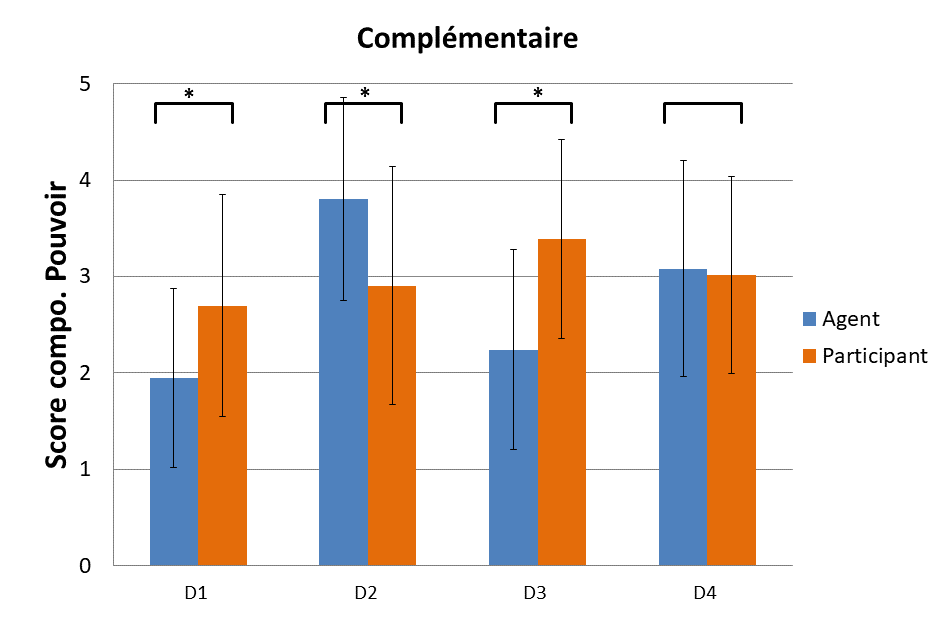
\includegraphics[clip=false]{Figures/chap7/comPow.PNG}
		}
		
		% this has a too narrow subfigure
		\subfloat[Moyenne et écart type dans les comportements de dominance]{
			\begin{tabular}{l c c c c c c}
				\hline\hline
				\textbf{Agent} & Evaluation&  \textbf{D1} & \textbf{D2} & \textbf{D3} & \textbf{D4} \\
				\hline
				
				\multirow{2}{*}{\textbf{Comp.} }& Moyenne & 1,94& 3,80 & 2,24 & 3,08 \\
				& Ecart-type & 0,93 & 1,05 & 1,03 & 1,11 \\
				
				\hline
				\multirow{2}{*}{\textbf{Part.}}& Moyenne & 2,69 & 2,94 & 3,4 & 3,02 \\
				& Ecart-type & 1,14 & 1,23 & 1,03 & 1,02\\
				\hline
				\hline
			\end{tabular}
		}
		\caption{Perception des comportements de dominance avec l'agent complémentaire}
		\label{fig:comp}
	\end{figure}	
	
	\subsubsection{Perception de similarité}
	Nous avons aussi analysé les comportements des négociateurs lors de leurs interactions avec l'agent Arthur. Les statistiques descriptives ont déjà montre une forte similarité dans la perception de tous les comportements (voir la figure \ref{fig:sim}). Nous avons complété l'étude par une comparaison de Wilcoxon a confirmé l'absence de différence significative comme présenté dans la table \ref{tab:domPercption}.  
	\begin{figure}[!tb]
		\centering
		% this is wide enough
		\subfloat[Score de perception des comportements de dominance]{
			\centering
			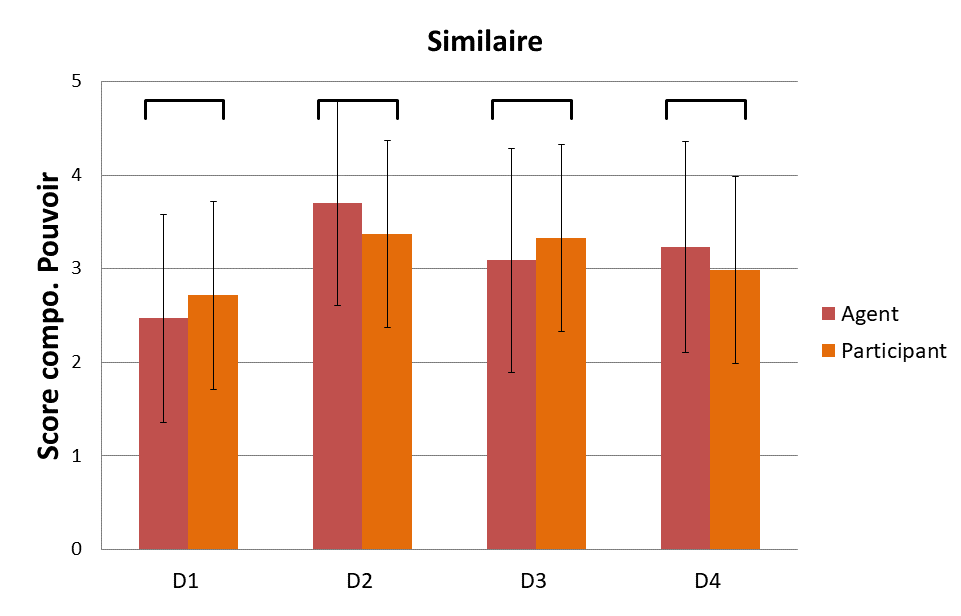
\includegraphics[clip=false]{Figures/chap7/simPow.PNG}
		}
		
		%\vspace{1em}
		% this has a too narrow subfigure
		\subfloat[Moyenne et écart type dans les comportements de dominance]{
			\centering
			\begin{tabular}{l c c c c c c}
				\hline\hline
				\textbf{Agent} & Evaluation& \textbf{D1} & \textbf{D2} & \textbf{D3} & \textbf{D4} \\
				\hline
				
				\multirow{2}{*}{\textbf{Simil.}}& Moyenne & 2,47 & 3,70 & 3,09 & 3,23 \\
				& Ecart-type & 1,11 & 1,10 & 1,19 & 1,12 \\
				
				\hline
				\multirow{2}{*}{\textbf{Part.}}& Moyenne & 2,71 & 3,37 & 3,33 & 2,98 \\
				& Ecart-type & 1,06 & 1,03 & 1,06 & 1,09\\
				\hline \hline
				
			\end{tabular}
		}
		\caption{Perception des comportements de dominance avec l'agent similaire Arthur}
		\label{fig:sim}
	\end{figure}
	
	\subsubsection{Comportement de l'agent neutre}
	
	Nous avons conduit les mêmes études statistiques pour analyser la perception des comportements de l'agent neutre. L'analyse descriptive présentée dans la figure \ref{fig:neutre} montre que les participants ont perçu que l'agent adoptait une stratégie complémentaire pour les comportements \textbf{D1}, \textbf{D2} et \textbf{D3}. Cependant, aucune différence significative n'a été perçu pour le comportement \textbf{D4}.
	
	\begin{figure}[!tb]
		\centering
		% this is wide enough
		\subfloat[Score de perception des comportements de dominance]{
			
			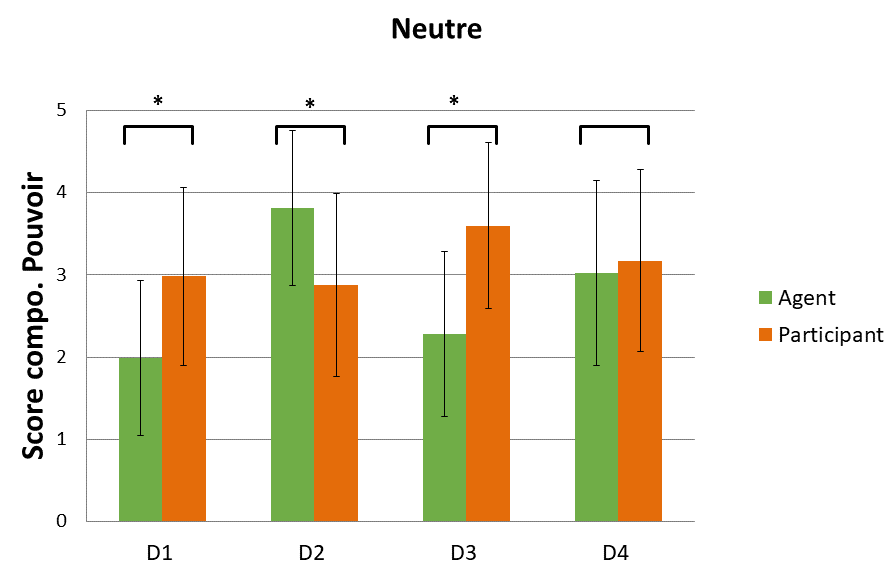
\includegraphics[clip=false]{Figures/chap7/neutrePow.PNG}
		}
		
		%\vspace{1em}
		% this has a too narrow subfigure
		\subfloat[Moyenne et écart type dans les comportements de dominance]{
			
			\begin{tabular}{l c c c c c c}
				\hline\hline
				\textbf{Agent} & Evaluation& \textbf{D1} & \textbf{D2} & \textbf{D3} & \textbf{D4} \\
				\hline
				
				\multirow{2}{*}{\textbf{Neutre}}& Moyenne & 1,99 & 3,81 & 2,28 & 3,02 \\
				& Ecart-type & 0,94 & 0,94 & 1,01 & 1,12 \\
				
				\hline
				\multirow{2}{*}{\textbf{Part}}& Moyenne & 2,98 & 2,88 & 3,60 & 3,17 \\
				
				& Ecart-type & 1,08 & 1,12 & 1,01 & 1,10 \\
				\hline \hline
				
			\end{tabular}
			
		}
		\caption{Perception des comportements de dominance avec l'agent neutre}
		\label{fig:neutre}
	\end{figure}
	
	\subsection{Gain commun}
	Nous avons analysé le gain commun des négociateurs durant les différentes négociations. Nous avons d'abord demandé aux participants leurs ressentis sur la satisfaction du restaurant choisi. Nous avons complété cette analyse par une étude objective dans laquelle nous avons calculé le score de satisfaction du restaurant choisi à partir des préférences du participant et de l'agent. L'ensemble des résultats est présenté en Annexe \ref{chap:Annexe}.
	
		\begin{figure}[h]
		
		\centering
		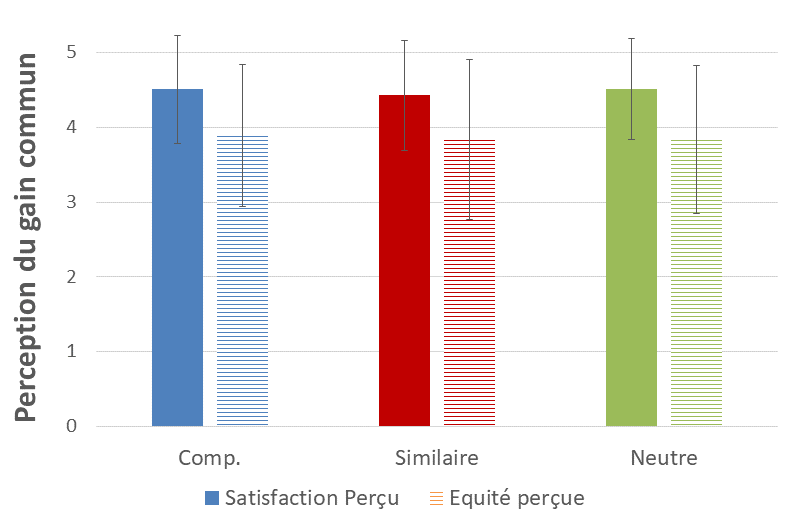
\includegraphics[width= 0.65 \linewidth,clip=false]{Figures/chap7/percpGain.PNG}
		\caption{Perception du gain commun obtenu pour tous les agents \textit{Aucune différence significative entre les agents}}
		\label{fig:gainCom}
	\end{figure}

	\subsubsection{Perception du gain commun} Nous avons demandé aux participants de renseigner leurs degrés de satisfaction du restaurant choisi avec l'agent.
	
	Les résultats sont présentés dans la figure \ref{fig:gainCom}. D'abord, les statistiques descriptives montrent qu'en moyenne les participants étaient satisfaits du restaurant choisi, et ce pour toutes les négociations. Les scores sont plutôt supérieurs à la moyenne pour tous les agents (les valeurs varient entre \emph{3.83} et \emph{4.5} sur une échelle de \emph{5}). 
	
	En outre, nous avons analysé si les participants étaient significativement plus satisfaits du restaurant choisi lors de la négociation avec l'agent Bob qu'avec les autres agents. Nous avons effectué un test de rangs signés de Wilcoxon car la normalité des données n'avait pu être assurée. L'analyse n'a montré aucune différence significative de la perception de gain et d'équité sur le choix du restaurant entre les différents agents. 
	
	\subsubsection{Analyse du gain commun } Concernant l'analyse objective du gain commun atteint à la fin de chaque négociation, nous avons dans un premier temps, récupéré les préférences des participants et des agents avec lesquels avaient interagi. 
	Ensuite, nous avons calculé la satisfiabilité du restaurant choisi pour chaque négociateur en fonction de leurs préférences (\textit{i.e. l'agent et le participant}). Nous avons ensuite, calculé le gain commun atteint à chaque négociation comme \textbf{la moyenne des valeurs de satisfiabilité} des deux négociateurs.  Les résultats obtenus pour chaque agent sont présentés dans la figure \ref{fig:gain}. 
	
		\begin{figure}[h]
		
		\subfloat[Score du gain commun atteint pour tous les agents  \textit{les populations regroupées avec $(*)$ sont significativement différentes }]{
			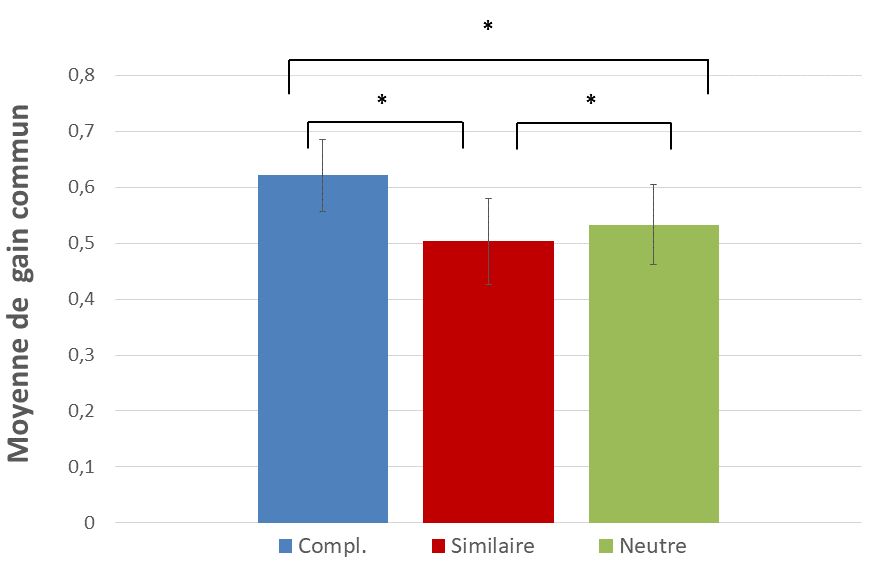
\includegraphics[clip=false]{Figures/chap7/gainCommun.PNG}}
		
		\subfloat [Score du gain commun obtenu par négociation]{
			\centering
			\begin{tabular}{l c c c}
				\hline
				\hline
				\textbf{ }& \textbf{Agent Comp.} & \textbf{Agent similaire} & \textbf{Agent neutre} \\ 
				\hline
				\newline Moyenne & 0.62& 0.5 & 0.53 \\
				\newline Écart type & 0.06 & 0.08 & 0.07 \\
				\hline
				\hline
			\end{tabular}
		}
		\caption{Les résultats obtenus pour le gain commun atteint durant la négociation}
		\label{fig:gain}
	\end{figure}

	Les valeurs de satisfiabilité sont supérieures à la moyenne pour tous les agents. Rappelons que les valeurs de satisfiabilité sont normalisées dans un intervalle $[0, 1]$. Nous avons étudié si les négociateurs avaient atteint un gain commun plus importants en négociant avec l'agent complémentaires comparés aux autres agents. En vue de la distribution normale des valeurs, nous avons appliqué un T-test afin de comparer chaque paire d'agents. Les résultats obtenus sont présentés dans la figure \ref{fig:gain}. L'analyse de la variance a montré une interaction significative entre la relation de dominance et le gain commun atteint lors des négociations. Effectivement, les participants ont atteint un gain commun significativement plus élevé en négociant avec l'agent complémentaire qu'avec l'agent similaire (\emph{t= 8.9, p < 0.01}). La même différence a été perçue en comparant avec l'agent neutre (\emph{t= 6.4, p < 0.01}).
	De plus, les participants ont atteint un meilleur gain commun avec l'agent neutre qu'avec l'agent similaire (\emph{t= 2.3, p = 0.02}).
	

	
	\subsection{Tours de paroles}
	
	Pour l'analyse de l'impact de la relation de dominance sur nombres de tours de paroles, nous avons recueilli le nombre de tours de paroles énoncé durant chaque négociation. Les statistiques descriptives sont présentées dans la figure \ref{fig:tour}. Un test paramétrique a été utilisée car les données suivent une distribution normale. Les résultats montrent que la négociation convergeait significative plus rapidement quand les participants négociaient avec l'agent complémentaire par rapport à l'agent similaire (\emph{t= 2.7, p = 0.003}). De même, la négociation convergeait plus rapidement avec l'agent neutre comparé à l'agent similaire (\emph{t= 4.43, p < 0.01}).  Les résultats sont présentés en Annexe \ref{chap:Annexe}.
	Cependant, aucune différence significative n'a été perçu entre l'agent complémentaire et l'agent neutre (\emph{t= 1.3, p = 0.09}).  
	
	\begin{figure}[!tbh]
		
		\subfloat[Nombre de tours de paroles durant une négociation pour tous les agents \textit{les populations regroupées avec $(*)$ sont significativement différentes}] {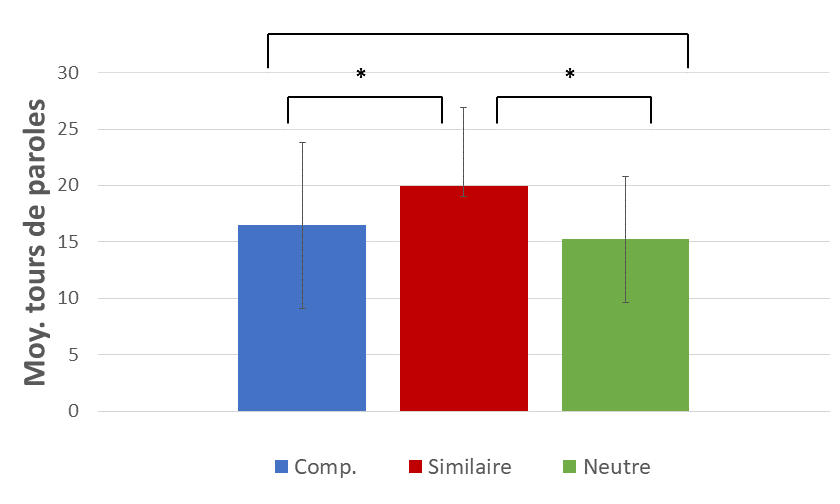
\includegraphics{Figures/chap7/tours.PNG}}
		
		
		\subfloat[Nombre de tours de paroles par négociation]{
			\centering
			\begin{tabular}{ l c c c }
				\hline
				\hline
				\textbf{ }& \textbf{Agent Comp.} & \textbf{Agent similaire} & \textbf{Agent neutre} \\ 
				\hline
				\newline Moyenne & 16.61& 19.94 & 15.13 \\
				\newline Écart type & 7.38 & 6.87 & 5.6 \\
				\hline
				\hline
			\end{tabular}
		}
		\caption{Résultats pour l'hypothèse H3.}
		\label{fig:tour}
	\end{figure}
	
	
	\subsection{Confort}
	
	Les statistiques descriptives sont présentées dans la table \ref{tab:confort}. Les participants se sont globalement sentis à l'aise avec tous les agents.
	Les score de détente ressentie sont au-dessus de 3,4 (sur une échelle à 5 points) pour tous les agents. Au contraire, les scores relatifs à l'anxiété  ressentie sont au-dessous de 2 (sur une échelle à 5 points) pour tous les agents. 
	
	Afin d'analyser une différence dans le confort perçue, nous avons utilisé un test non paramétrique car la normalité n'a pas pu être assurée. Le test de rang signé de Wilcoxon a été appliqué afin d'analyser si les participants se sont sentis plus à l'aise avec l'agent complémentaire qu'avec les autres agents. (Voir résultats en annexe \ref{chap:Annexe}). 
	Les résultats montrent que les participants se sont sentis plus à l'aise avec l'agent complémentaire qu'avec l'agent similaire (\emph{Z= -2.73, p = 0.002})
	avec un effet de taille faible (\emph{e = -0.1}). Cependant, aucune différence significative n'a été perçu entre l'agent complémentaire et l'agent neutre. 
	
	
	\begin{figure}[h]
		
		\subfloat[Score de confort que les participants ont ressenti pour tous les agents. \textit{les populations regroupées avec $(*)$ sont significativement différentes }]{
			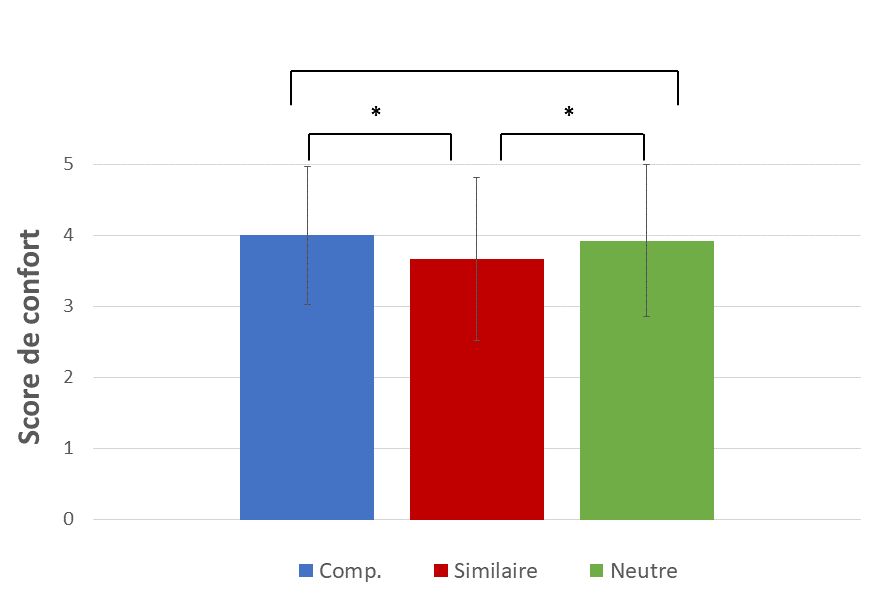
\includegraphics[clip=false]{Figures/chap7/confort.PNG}
		}
		
		\subfloat[L'effet de la relation de dominance sur le confort ressenti pendant la négociation avec l'agent]{
			\centering
			\begin{tabular}{ l l c c c  }
				\hline\hline
				\textbf{ }& & \textbf{Agent Comp.} & \textbf{Agent similaire} & \textbf{Agent neutre} \\ 
				\hline
				\newline \newline\multirow{2}{*} {Détendu} & Moy. &3.79 & 3.47 & 3.79 \\
				\newline  & SD & 1 & 1.2 & 1 \\
				\hline
				
				\newline \newline\multirow{2}{*} {Anxieux} & Moy. & 1.79 & 2.13 & 1.93 \\
				\newline  & SD & 7.38 & 6.87 & 5.6 \\
				\hline\hline
			\end{tabular}
		}
		\caption{Résultats pour la perception du confort durant la négociation.}
		\label{tab:confort}
	\end{figure}	
	\vspace{- 1 em}
	
	\subsection{Appréciation}
	Les statistiques descriptives concernant les scores d’appréciation sont présentées dans la figure \ref{fig:app}. Globalement,
	les scores sont centrés autour de 3.7 (sur une échelle de 5). L'analyse de variance montre l'effet de la relation de dominance sur la perception de l'appréciation. Les résultats sont présentés en annexe \ref{chap:Annexe}.
	
	\begin{figure}[h]
		
		\subfloat[Score d'appréciation perçue pour tous les agents. \textit{les populations regroupées avec $(*)$ sont significativement différentes}]{
			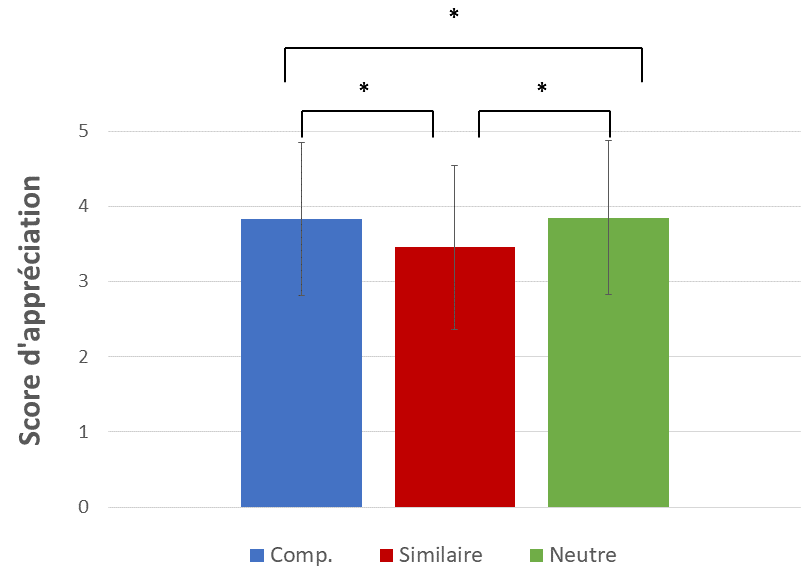
\includegraphics[clip=false]{Figures/chap7/appreciation.PNG}
		}
		
		\subfloat[L'effet de la relation de dominance sur l'appréciation perçue]{			
			
			\begin{tabular}{ l c c c c c }
				\hline\hline
				\textbf{ }& \textbf{Agent Comp.} & &  \textbf{Agent similaire} & & \textbf{Agent neutre} \\ 
				\hline
				\newline Moy. & 3.83 & &3.46 & & 3.85 \\
				\newline SD & 1.01 & & 1.09& &  1.02 \\
				\hline\hline
				
			\end{tabular}
		}
		\caption{Résultats pour la perception de l'appréciation.}
		\label{fig:app}
	\end{figure}
	
	
	Le test de rangs signé de Wilcoxon montre que l'agent complémentaire a été perçu comme significativement plus agréable que l'agent similaire (\emph{p < 0.01, Z = -3.17}). Par ailleurs, l'agent neutre a aussi été perçu comme plus agréable que l'agent similaire (\emph{p < 0.01, Z = -3.3}). Cependant, aucune différence n'a été perçu entre l'agent complémentaire et l'agent neutre (\emph{p = 0.6, Z = -0.31}).
	
	Nous nous sommes aussi intéressés à la facilité de collaboration entre le participant et l'agent. En effet, nous avons demandé aux participants de relater le degré de facilité de négociation avec l'agent. Les résultats sont présentés dans la figure \ref{fig:aise}. En général, les participants ont trouvé que la négociation été aisée avec l'agent complémentaire (\emph{M= 4, SD = 1}) ainsi qu'avec l'agent neutre (\emph{M=3.9, SD =0.99}). Les participants ont perçue la négociation avec l'agent similaire comme moins aisée (\emph{M=3.16, SD = 1.06}). 
	Nous avons ensuite analysé si cette différence de perception été significative. Comme les données ne sont pas normalement distribué, nous avons appliqué le test de rangs signé de Wilcoxon. Les résultats montrent qu'en effet les participants ont trouvé que négocier avec l'agent similaire été significativement moins aisée comparé à l'agent complémentaire (\emph{p < 0.01, Z = -3.86} avec un effet de taille moyen \emph{e = -0.35}) et l'agent neutre (\emph{p < 0.01, Z = -3.61} avec un effet de taille moyen \emph{e = -0.32}).
	Cependant, aucune différence n'a été perçue entre l'agent complémentaire et l'agent neutre.
	\begin{figure}[h]
		
		\subfloat[Évaluation de la collaboration durant la négociation. \textit{les populations regroupées avec $(*)$ sont significativement différentes }]{
			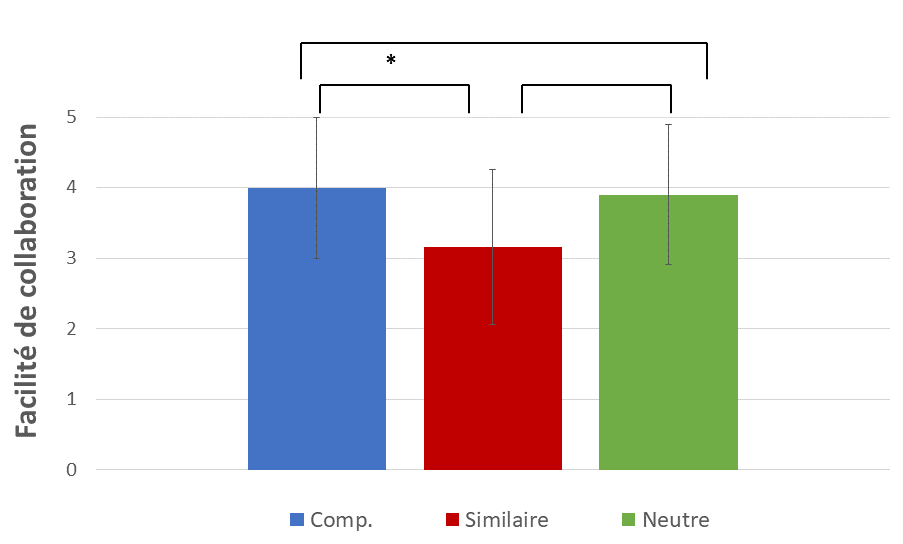
\includegraphics[clip=false]{Figures/chap7/aisee.PNG}
		}
		
		\subfloat[L'effet de la relation de dominance sur la facilité de collaboration]{
			\centering
			\begin{tabular}{ l c c c c c }
				\hline\hline
				\textbf{ }& \textbf{Agent Comp.} & &  \textbf{Agent similaire} & & \textbf{Agent neutre} \\ 
				\hline
				\newline Moy. & 4 & & 3.16 & & 3.9 \\
				\newline SD & 1 & & 1.09  & & 0.99   \\
				\hline\hline
				
			\end{tabular}
		}
		\caption{Résultats pour la facilité de collaboration durant la négociation.}
		\label{fig:aise}
	\end{figure}
	
	
	\section{Analyses complémentaires}
	Dans le chapitre 2, nous présentons la relation de dominance comme une relation interpersonnelle qui s'établie durant l'interaction. 
	Par conséquent, en plus du trais de personnalité, un individu est influencé par l'environnement de l'interaction (\textit{ex.} contexte de l'interaction, rôle social ...). Ces différents paramètres vont créer une certaine relation de dominance qui peut varier d'une interaction à une autre.  
	Afin de vérifier si les participants produisaient différents comportements de dominance durant les différentes négociations, nous avons recueilli la perception de l'agent des comportements de dominance de son interlocuteur.  Les résultats sont présentés dans la figure \ref{fig:dom}.
	
	Nous avons analysé, pour le même participant, la variance des comportements de dominance à travers les trois négociations. Pour ce faire, nous avons utilisé le test de rang signé de Wilcoxon car la normalité des données n'a pu être assurée. 
	
	Les résultats montrent les comportements de dominance des participants variaient d'une interaction à une autre. En effet, le test de Wilcoxon révèle une différence significative entre les comportements perçus par l'agent complémentaire et l'agent similaire (\emph{p<0.01, Z = -3.35}). Ces mêmes résultats sont observés en comparant la perception de l'agent complémentaire et l'agent neutre (\emph{p< 0.01, Z = -3.88}).
	Toutefois, aucune différence entre l'agent similaire et l'agent neutre n'a été vérifié (\emph{p = 0.6, Z = 0.44}). 
	
	Ces résultats suggèrent que les participants ont adopté une stratégie de négociation différente en fonction de la relation établie avec l'agent. 
	
	\begin{figure}[h]
		
		\subfloat[Évaluation de comportements de dominance des participants perçus par les agents. \textit{les populations regroupées avec $(*)$ sont significativement différentes }]{
			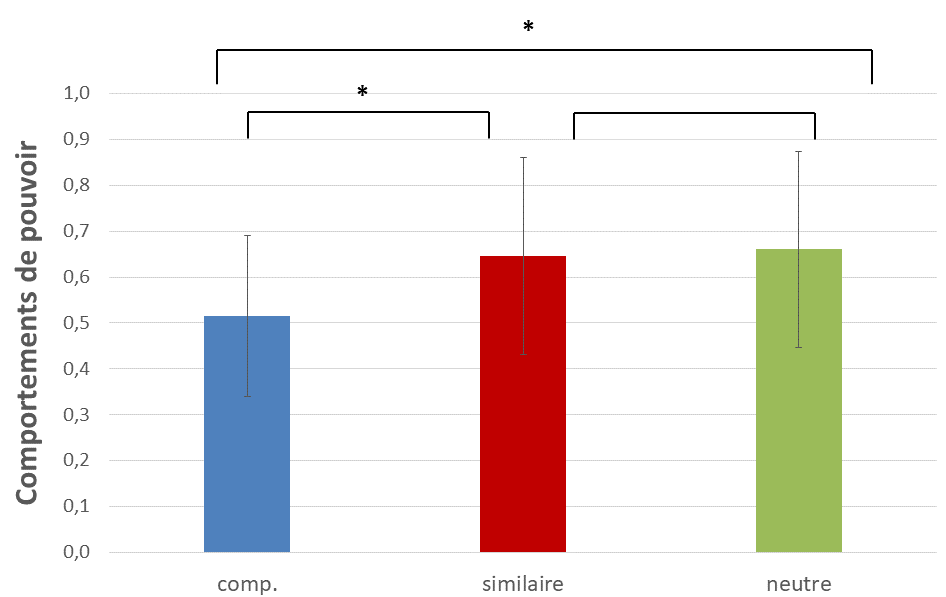
\includegraphics[clip=false]{Figures/chap7/pow.png}
		}
		
		\subfloat[Perception de l'agent des comportements de dominance exprimés par les participants]{
			\begin{tabular}{ l c c c c c }
				\hline
				\hline
				\textbf{ }& \textbf{Agent Comp.} & &  \textbf{Agent similaire} & & \textbf{Agent neutre} \\ 
				\hline
				\newline Moy. & 0.51 && 0.64 && 0.66 \\
				\newline SD & 0.17 && 0.21 && 0.219   \\
				\hline
				\hline
			\end{tabular}
		}
		\caption{Résultats pour la variation des comportements de dominance à travers les interactions.}
		\label{fig:dom}
	\end{figure}
	
	\section{Discussion}
	\label{sec:discussion}
	En général, toutes nos hypothèses ont été validées. Ces résultats appuient la validité de notre modèle négociation collaborative et de théorie de l'esprit dans le cadre d'une interaction agent/humain.   
	
	\subsection{Perception des comportements des agents}
	Notre hypothèse H1 (\textit{les comportements de complémentarité et de similarité des agents virtuels sont perçus par les participants}) est partiellement validée. 
	
	Quatre comportements de dominance ont été pris en compte pour mesurer la stratégie de négociation. 
	Les participants ont été en mesure de distinguer une différence significative de trois comportements sur quatre entre leurs stratégies et celle de l'agent complémentaire.
	
	En effet, les participants ont perçu une différence entre leurs niveaux d'exigences et de concessions \textbf{D3}, \textbf{D2}, ainsi que la prise en compte des préférences de l'autre \textbf{D1}. Cependant, aucune différence n'a été perçu concernant les comportements de leadership durant la négociation \textbf{D4}. 
	
	Concernant, les comportements de l'agent neutre, ce dernier a été perçu comme significativement complémentaires aux utilisateurs pour les comportements \textbf{D1}, \textbf{D2} et \textbf{D3}. 
	Toutefois, comme l'agent complémentaire, aucune différence n'a été perçue dans les comportements relatifs à \textbf{D4} entre l'agent neutre et les participants. 
	
	Nous avons étudié les données afin de comprendre pourquoi les participants ne percevaient pas de différence dans les comportements de leadership. 
	
	Concernant l'agent complémentaire, les comportements de leaderships ont pu être masqué à cause de  sa stratégie d'adaptation qui modifié ses comportements de dominance à chaque tour de parole.
	
	En outre, l'aspect collaboratif de la négociation pourrait avoir atténué la perception du leadership dans la négociation ce qui pourrait expliquer le cas de l'agent neutre. 
	
	Enfin, l'absence de résultats pour les deux agents nous amènent à nous questionner sur les items proposés pour mesurer le leadership. 
	Il serait intéressant de faire une évaluation post-hoc afin de demander aux participants le types de comportements qu'identifieraient le leadership durant la négociation.
	
	En parallèle, les participants ont perçu une similarité entre leurs comportements et ceux de l'agent similaire. En moyenne, pour chaque comportement, les valeurs assignés en auto-attribution et en hétéro sont très proches. De plus, l'absence de différence significative appuie ce résultat. Nous sommes conscients que l'absence de différence n'est pas une assurance de similarité de perception. Cependant, il est difficile de trouver un calcul statistique qui assure la similarité entre deux populations.
	
	D’un point de vue plus général, les résultats obtenus appuient la cohérence de notre modèle de décision tant sur la perception des comportements de dominance que sur la capacité de l'agent à percevoir les comportements de son interlocuteur et de s'y adapter correctement.  
	
	Par ailleurs, la perception des comportements de l'agent neutre comme complémentaires à ceux des participants soutient que la relation interpersonnelle de dominance qui s'établie au cours de l'interaction est complémentaire \cite{burgoonnonverbal}. En effet, indépendamment des deux autres agents où nous avions manipulé l'adaptation de l'agent, dans la condition neutre l'agent ne s'adapte pas aux comportements du participant. Néanmoins, les résultats démontrent que le participant s'est adapté aux comportements exhibés par l'agent et a ainsi établie une relation interpersonnelle de dominance complémentaire.
	
	\subsection{Gain commun}
	Notre seconde hypothèse (\textit{Les négociateurs atteignent un gain commun plus important quand les négociateurs établissent une relation de dominance complémentaire.}) est validée. 
	
	Nous avons en premier temps demandé aux participants de relater leur avis sur le restaurant choisi pour chaque négociation.
	En général, les participants ont été satisfaits du choix final et le trouvaient équitable pour toutes les négociations. 
	En analysant la valeur de satisfiabilité du restaurant choisi pour les préférences des participants (voir table \ref{tab:gainPerceptif}), les valeurs étaient autour de 0.7 (\emph{min =0.69, max = 0.73}). 
	
	Cependant, en analysant la valeur de satisfiabilité pour les préférences de l'agent,  en moyenne, seul l'agent complémentaire a pu converger vers un restaurant qui respecte ses préférences (\emph{M = 0.53, SD = 0.2}). 
	
	
	\begin{table}
		\centering
		\caption{Moyenne des valeurs de satisfiabilité du restaurant choisi pour chaque négociateur} 
		\begin{tabular} {lcccccccc}
			\hline
			\hline
			& \multicolumn{2}{c}{Agent Comp.} & & \multicolumn{2}{c}{Agent similaire}& & \multicolumn{2}{c}{Agent neutre} \\ % column 4 blank, for spacing
			\cline{2-3} \cline{5-6} \cline{8-9} % horizontal lines connecting cols. 2-3, 5-6
			& Part. & Agent & & Part. & Agent & &  Part. &Agent \\ \hline
			Moy. &0,71 & 0,53 & &  0,69 & 0,33 & & 0,73 & 0,34 \\
			SD & 0,2 & 0,24 & &  0,18 & 0,19 & & 0,18 & 0,16 \\
			\hline
			\hline
		\end{tabular}
		\label{tab:gainPerceptif}
		
	\end{table}
	
	Concernant l'agent similaire, la moyenne de satisfiabilité est assez basse. Ceci est causé par le fait que les négociateurs ne communiquaient pas bien durant la négociation. Par conséquent, la négociation durait plus longtemps causant la chute de la courbe de concession $Self$. De ce fait, l'agent faisait plus de concession et finissait par accepter un restaurant dont la satisfiabilité n'était pas élevée (\emph{M = 0.33, SD = 0.18}).
	
	Concernant l'agent neutre qui n'est pas très dominant, il est normal que dans la majorité des cas, la courbe de concession finissait par décroitre menant l'agent à faire des concessions importantes. Ceci explique la moyenne de satisfiabilité atteinte par l'agent neutre  (\emph{M = 0.34, SD = 0.16}).
	
	Cette analyse confirme les résultats de l'étude objective menée.
	Pour toutes les négociations, nous avons comparé le gain commun et nous avons observé qu'il était significativement plus important durant les négociations avec l'agent complémentaire comparé aux autres agents. De plus, les négociateurs avaient de meilleurs gains durant la négociation avec l'agent neutre comparé à l'agent similaire. Ceci prouve que la relation complémentaire qui s'est installé durant la négociation avec l'agent neutre a permis un meilleur échange d'information. 
	
	Ces résultats confirme que les négociateurs communiquent mieux et par conséquent négocient mieux dans le cadre d'une relation complémentaire de dominance.  
	
	
	\subsection{Tours de paroles}
	Notre hypothèse H3 (\textit{La négociation converge plus rapidement dans le cas où les négociateurs ont une relation de dominance complémentaire}) est validée. En effet, la négociation convergeait en moyenne plus rapidement quand une relation de dominance complémentaire s'établissait entre l'agent et le participant. De plus, dans cette même condition le gain commun atteint par les négociateurs était plus important. Ainsi, ces résultats appuient les théories de  psychologie sociales selon lesquelles la relation interpersonnelle de dominance améliore la coordination et l'échange d'informations.
	
		
	En ce qui concerne l'agent neutre, la négociation convergeait rapidement à cause de deux raisons. Premièrement, avec une valeur de dominance initialisée à 0.5, l'agent avait un niveau d'exigence moyen ce qui facilitait le processus pour trouver un compromis. 
	Deuxièmement, d'après nos résultats, dans cette condition, une relation complémentaire de dominance s'était établie entre les négociateurs ce qui facilitait la coordination. 
	
	En conclusion, la relation interpersonnelle de dominance améliore la coordination et l'échange d'information qui résulte en des processus de négociation court et plus efficaces. 
	
	\subsection{Appréciation de l'agent}
	Nos hypothèses H4 (\textit{Le négociateur se sent plus à l'aise avec un partenaire qui exprime un comportement complémentaire})  et H5  (\textit{La complémentarité dans la relation de dominance augmente l'appréciation entre les négociateurs.}) sont validées. 
	
	Pour l’appréciation, les scores sont au-dessus de la moyenne pour tous les agents. Ce pourrait être le reflet d’un léger biais positif envers les agents. Toutefois, l'analyse des différences a révélé que les participants ont significativement plus apprécié la négociation avec l'agent complémentaire que l'agent similaire. De même, les participants ont jugé que l'agent neutre était aussi plus agréable que l'agent similaire. 
	
	En outre, nous avons analysé le confort ressenti lors de la négociation. Globalement, les participants se sont sentis détendus durant la négociation et ont trouvé la négociation confortable avec tous les agents.  
	
	L'analyse de variance a révélé que les participants se sont plus sentis à l'aise avec l'agent complémentaire qu'avec l'agent similaire. Cependant, aucune différence n'a été perçu entre l'agent complémentaire et l'agent neutre, et entre l'agent neutre et l'agent similaire.
	
	En plus du confort, nous avons analysé la facilité de collaborer avec l'agent durant la négociation. Les résultats montent que les participants ont perçu le processus de négociation comme plus aisé avec l'agent complémentaire et l'agent neutre qu'avec l'agent adoptant une stratégie similaire à la leurs. 
	
	Ces résultats confirment nos hypothèses. Les participants préfèrent négocier avec un partenaire avec lequel ils ont établi une relation complémentaire qu'avec un négociateur qui exhibe des comportements de dominance similaires. 
	
	
	\section{Conclusion}
	Pour cette quatrième étude, nous avions pour objectif d'étudier l'effet de la relation de dominance sur la négociation entre un agent et un participant humain. Nous nous sommes basés sur les travaux de Tienders et Wiltermuth \cite{wiltermuth2009benefits,tiedens2003power} qui affirment que la complémentarité dans la relation de dominance avait un impact positif sur la négociation. 
	
	Nous avons implémenté trois agents négociateurs adoptant trois stratégies différentes, un agent complémentaire, un agent similaire et un agent neutre. 
	63 participants ont pris part à  des négociations collaboratives avec ces agents dans le but de trouver un restaurant qui satisfassent leurs préférences. 
	
	Les résultats ont confirmé la majorité de nos hypothèses et nous ont permis d'aller plus loin dans l'analyse des comportements de dominance dans la négociation. 
	
	D'abord, nous avons pu valider notre modèle de la théorie de l'esprit dans le cadre d'une interaction avec un utilisateur humain. 
	Les résultats montrent que les participants ont été capables de percevoir une différence dans les stratégies qu'adoptaient les agents. Ceci nous permet de valider la robustesse des prédictions de notre modèle. 
	
	Par ailleurs, toutes les hypothèses relatives à l'effet positif de la relation de dominance complémentaire ont été validées. Quand les négociateurs établissaient une relation de dominance complémentaire, ils atteignaient un meilleur gain commun et ceux dans un délai plus court comparés aux autres configurations. La négociation était vécue comme plus agréable et confortable et les négociateurs semblaient mieux collaborer. 
	
	Les résultats ont aussi révélé des comportements qui soutiennent les travaux en psychologie sociale. En effet, en analysant les comportements exprimés lors des négociations avec l'agent neutre, nous nous sommes rendu compte qu'une relation complémentaire de dominance s'était installé entre les négociateurs. Ces résultats appuient la définition de Dunbar and Burgoon \cite{dunbar2005perceptions} qui affirment que la relation de dominance est forcément complémentaire. En outre, la relation de dominance étant interpersonnelle, elle s'établie durant l'interaction. Ce point a aussi été validé par nos analyses qui nous ont permis de montrer que les participants ont adopté des comportements de dominance différents d'une négociation à une autre. Cela suggère que les négociateurs s'adaptent à leur interlocuteur pour définir une relation de dominance propre à l'interaction. 
	%\chapter{Processus de décision basé sur le pouvoir}
	%		\label{chap:dec}
%	\chapter{Annexe}
%
%		\begin{appendix}


\section{Gain commun atteint dans la négociation}

	\subsection{Perception du gain commun}

\begin{table} [h]
	
	\begin{tabular}{ l c c c c }
		\hline\hline
		\textbf{ }& & \textbf{Comp. >Similaire} & \textbf{Comp. >Neutre} & \textbf{Neutre >Similaire} \\ 
		\hline
		
		
		\multirow{3}{*} {Équité}  &  T-test  & \\ 	
		& p-value & \\ 
		\hline
		
		\multirow{3}{*} {Satisfaction}  &   T-test  &  &  &   \\ 	
		& p-value &  &   &   \\ 
		\hline
	\end{tabular}
	\caption{Analyse du gain commun atteint par tous les agents}
\end{table}

\subsection{Satisfaction du choix final}

	\begin{table}[h]
		
		\begin{tabular}{ c c c c }
			\hline\hline
			 & \textbf{Comp. >Similaire} & \textbf{Comp. >Neutre} & \textbf{Neutre >Similaire} \\ 
			\hline \hline
			
				  T-test  & 8,9 & 6,4 &  2,3 \\ 	
				p-value & 1,74E-12 &  2,884E-08 & 0,025  \\ 
			\hline
			\hline
			
			
			
		\end{tabular}
		\caption{Analyse du gain commun atteint par tous les agents}
	\end{table}
\vspace{-1 em}

\section{Tours de paroles par négociation}

\begin{table}[t]
	
	\begin{tabular}{ c c c c }
		\hline\hline
		& \textbf{Comp. < Similaire} & \textbf{Comp. < Neutre} & \textbf{Neutre < Similaire} \\ 
		\hline\hline
		
		T-test  & 3.33 & 1.49 &  5.56 \\ 	
		p-value & 0.0007 &  0,06 & 2.595e-07 \\ 
		\hline
		\hline
	
		
		
	\end{tabular}
	\caption{Analyse du gain commun atteint par tous les agents}
\end{table}


\section{Appréciation et confort durant la négociation}

\begin{table}[h]
			\centering
	\begin{tabular}{ l c p{3 cm} p{3 cm} p{3 cm} }

		\hline\hline
		\textbf{ }& & \textbf{Comp.>Sim.} & \textbf{Comp.>Neutre} & \textbf{Neutre>Sim.} \\ 
		\hline
		
		\multirow{3}{*} {Appréciation}  & Z-Wilcoxon& -3,17 & -0,32 & -3,29	\\ 	
										& p-value &	0,0005 & 0,6298 & 0,0003  \\ 
										& Effect size & -0,20 & -0,02 & -0,21 \\ 
		\hline
		
		\multirow{3}{*} {Confort}  &Z-Wilcoxon& -2,74 & -0,81 & -2,62 \\
									& p-value & 0,0026 & 0,2 & 1 \\ 
									& Effect size & -0,18 & -0,05 & -0,17 \\ 
		
		
		\hline\multirow{3}{*} {Collaboration}  &  Z-Wilcoxon  & -3,86 & -0,91 & -3,61\\ 	
		& p-value & 4,28E-05 & 0,1718 & 0,0001\\ 
		& Effect size & -0,35 & -0,08 & -0,33 \\ 
		\hline
		\hline
		
	\end{tabular}
	\caption{Les scores d'appréciation pour tous les agents}
\end{table}
\end{appendix}



%			\label{chap:Annexe}

	\bibliographystyle{abbrv}
	\bibliography{Library}
\end{document}